\chapter{Trilepton Resonance Search}\label{ch:trilepton-resonance-search}

\section{Motivation}
This note documents a search for new heavy leptons, $\lpm$, decaying resonantly into a trilepton final state. The search is motivated by two avenues of phenomena beyond the Standard Model: the type III neutrino seesaw model and extra generations of vector-like leptons. The models both propose heavy, charged, and colorless fermions which are made unstable via mixing with Standard Model leptons. The mixing gives rise to the decay $\lpm\rightarrow Zl^{\pm} \rightarrow l^{\pm} l^{\mp} l^{\pm}$. If all three leptons are electrons or muons, the signature of this decay is a narrow trilepton resonance, where two of the leptons are consistent with the decay of an on-shell $Z$ boson. The fully reconstructible decay gives a powerful constraint with which to reduce backgrounds. 

In the models considered here, the heavy leptons are either pair produced, $pp\rightarrow \Sigma^+\Sigma^-$, or produced in association with a heavy neutral fermion, $pp\rightarrow \lpm\Sigma^0$. In order not to be stable, the heavy leptons are hypothesized to mix with one or more Standard Model leptons, so the physical mass eigenstates decay to a massive boson ($W$, $Z$, or $h$) and a lepton or a neutrino. Feynman diagrams for the production and decay of the heavy leptons are shown in figure~\ref{fig:heavy-lepton-feynman-diagrams}. The branching ratios are shown in figure~\ref{fig:branching-ratios}. The asymptotic values as $m_{\lpm}\rightarrow \infty$, $\mathcal{B}(\lpm\rightarrow W^{\pm}\nu)=50\%$, $\mathcal{B}(\lpm\rightarrow Zl^{\pm})=25\%$, and $\mathcal{B}(\lpm\rightarrow hl^{\pm})=25\%$, are predicted by the Goldstone boson equivalence theorem~\cite{Chanowitz1985379}. 

\begin{figure}[h]
  \centering
  \subfloat[ Pair production of charged heavy leptons.] {
    \resizebox{0.45\textwidth}{!}{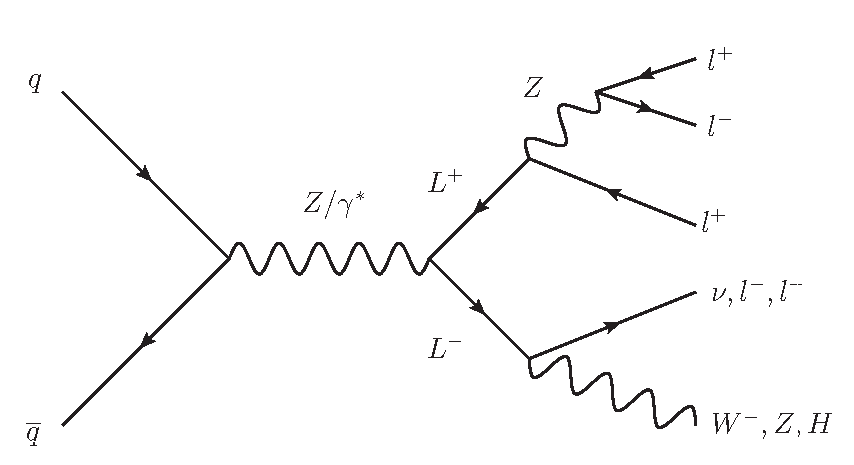
\includegraphics{figures/ch7-resonance/fd_cc2.eps}}
    \label{fig:heavy-lepton-feynman-diagrams-cc}
  }
  \subfloat[ Production of a charged and a neutral heavy lepton.] {
    \resizebox{0.45\textwidth}{!}{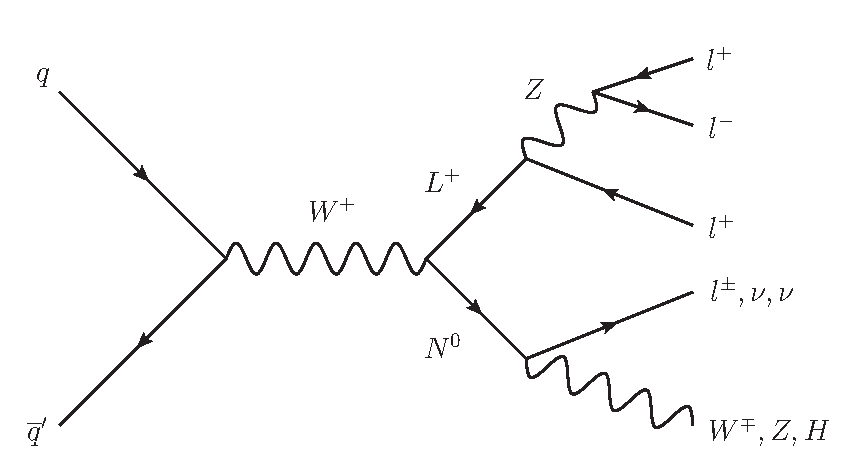
\includegraphics{figures/ch7-resonance/fd_cn2.eps}}
    \label{fig:heavy-lepton-feynman-diagrams-cn}
  }
  \caption{Production and decay of new heavy leptons to final states with a trilepton resonance.}
  \label{fig:heavy-lepton-feynman-diagrams}
\end{figure}


\begin{figure}[h]
  \centering
  \subfloat[ Charged heavy fermion] {
    \resizebox{0.45\textwidth}{!}{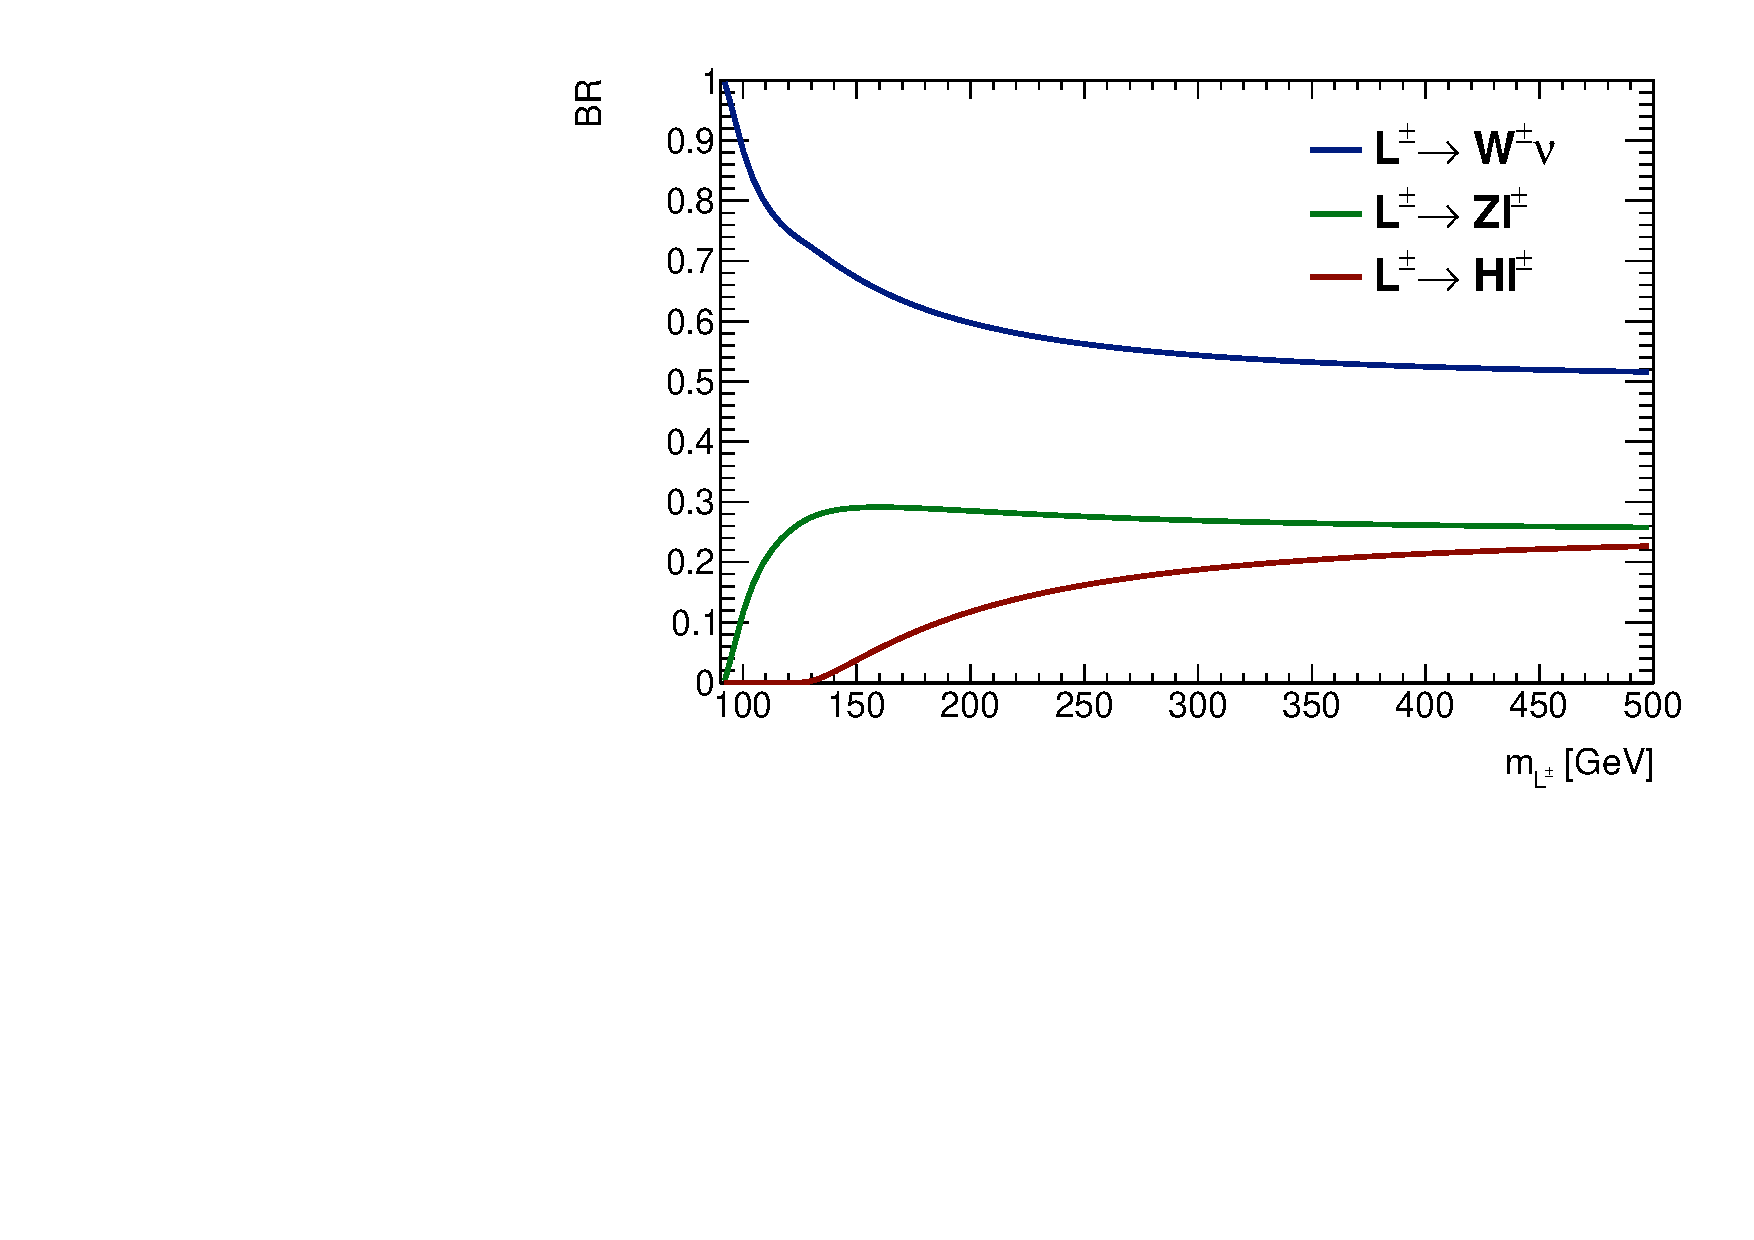
\includegraphics{figures/ch7-resonance/c_br_charged}}
  }
  \subfloat[ Neutral heavy fermion] {
    \resizebox{0.45\textwidth}{!}{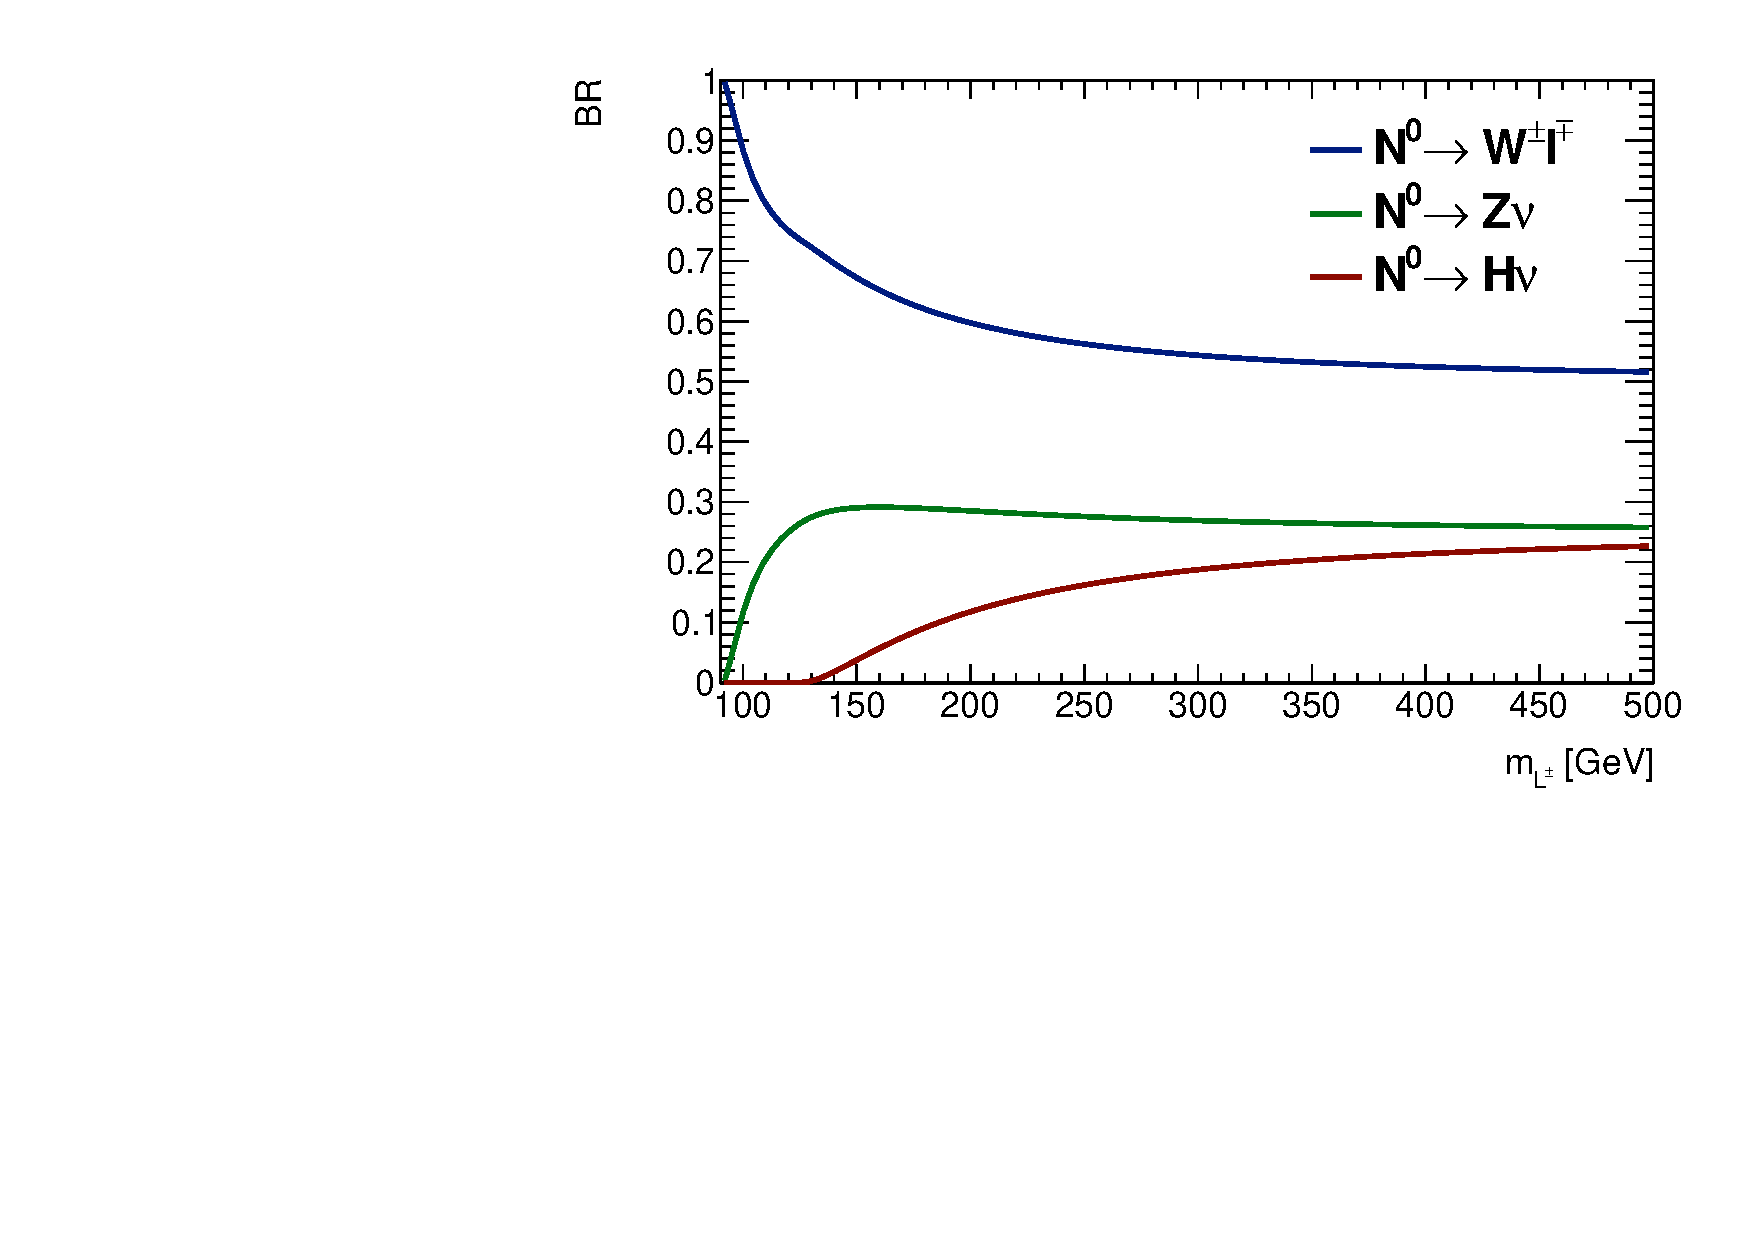
\includegraphics{figures/ch7-resonance/c_br_neutral}}
  }
  \caption{Branching ratios of a heavy lepton decaying via mixing with Standard Model leptons~\cite{Biggio:2011ja}.}
  \label{fig:branching-ratios}
\end{figure}




\subsection{Common Aspects of New Heavy Leptons}
A review of extra fermion generations beyond the Standard Model is presented in~\cite{Frampton:1999xi}. Motivations for extra generations of fermions include:

\begin{itemize}
  \item The quadratic Higgs mass divergence can be regulated with the addition of a vector-like top quark partner~\cite{DeSimone:2012fs}. 
  \item Grand unified theories with gauge groups larger than $\mathrm{SU}(5)$ contain additional matter content. 
  \item In supersymmetric contexts, additional vector-like supermultiplets can contribute positively the Higgs mass, which can alleviate fine tuning problems~\cite{Hall:2011aa, Martin:2009bg}.
  \item The type III neutrino seesaw model creates the dimension-5 operator associated with the neutrino mass suppression using an $\mathrm{SU}(2)_L$ triplets of fermions.
\end{itemize}

The models considered here posit one or more new charged, colorless fermions (heavy leptons, $\lpm$), and zero or more neutral, colorless fermions (heavy neutrinos, $\lzero$). The $\mathrm{SU}(2)$ representations of the new particles varies between models.

The new particles are pair produced via gauge interactions, $q\overline{q}\rightarrow \lpm\lmp$ or $q\overline{q}'\rightarrow \lpm\lzero$, as shown in figure~\ref{fig:heavy-lepton-feynman-diagrams}. The production cross sections depend on how the new particles couple to $\mathrm{SU}(2)_L\times \mathrm{U}(1)_Y$; for example, the type III seesaw fermions transform in the adjoint representation of $\mathrm{SU}(2)_L$ and have zero hypercharge, $(\mathbf{3},\ 0)$, while the heavy lepton in the generic vector-like lepton model inherits its gauge couplings from its $\mathrm{SU}(5)$ multiplet, $(1,\ -1)$.  The different gauge couplings, plus the various production modes, lead to significant differences in production rates, as described in later sections.

The heavy leptons are made unstable by introducing mixing terms with the Standard Model leptons. For example, consider a single extra generation of fermions transforming in the adjoint representation of $\mathrm{SU}(2)_L$, as in the type III seesaw model: $\Sigma\equiv \left(\begin{array}{cc} \lzero/\sqrt{2} & \Sigma^+ \\ \Sigma^- & -\lzero/\sqrt{2}\end{array}\right)$~\cite{Abada:2008ea,Biggio:2011ja}. The Lagrangian contains Yukawa terms mixing the heavy leptons with Standard Model leptons:
\begin{equation}
  -\mathcal{L} \ni \sum_{l=e,\mu,\tau} \sqrt{2}\phi^0 \overline{\Psi} Y_{\lpm l} l_L + \mathrm{h.c.},
\end{equation}
where $\Psi\equiv \Sigma^{+c}_R + \Sigma^-_R$ is a Dirac spinor representating the four charged degrees of freedom, $\phi\equiv(\phi^+,\phi^0)^T\equiv (\phi^+,(v+H+i\eta)/\sqrt{2})^T$ is the Higgs doublet, $Y_{\lpm l}$ are Yukawa couplings, and $l_L$ is a Standard Model lepton. After electroweak symmetry breaking, the mass matrices take the form
\begin{equation}
-\mathcal{L} \ni \sum_{l=e,\mu,\tau} \left(\begin{array}{cc}\overline{l}_R & \overline{\Psi}_R \end{array} \right) \left(\begin{array}{cc} m_l & 0 \\ Y_{\lpm l}v & M_{\lpm} \end{array}\right) \left(\begin{array}{c} l_L \\ \Psi_L \end{array}\right)  + \left(\begin{array}{cc}\overline{l}_L & \overline{\Psi}_L\end{array}\right) \left(\begin{array}{cc} m_l & Y_{\lpm l}^{\dagger}v \\ 0 & M_{\lpm} \end{array}\right) \left(\begin{array}{c} l_R \\ \Psi_r \end{array}\right).
\end{equation}

Diagonalizing the mass matrices leads to off-diagonal terms in the gauge interactions, with couplings proportional to the mixing parameters $V_{\alpha\Sigma}=\frac{v}{\sqrt{2}} M_{\lpm}^{-1} Y_{\alpha\Sigma}$. These couplings enable the decay of the heavy leptons to a boson ($W$, $Z$, or $h$) plus a Standard Model lepton or neutrino, with partial widths given by:

%
\begin{align}
\label{eq:Gammatr0W}
\Gamma(\lzero \to l_\alpha^- W^+) &=  \Gamma(\lzero \to l_\alpha^+ W^-) =
\frac{g^2}{64 \pi} |V_{\alpha\Sigma}|^2
\frac{M_{\lpm}^3}{M_W^2} \left( 1- \frac{M_W^2}{M_{\lpm}^2} \right)^2 
\left( 1 + 2 \frac{M_W^2}{M_{\lpm}^2} \right) , 
\\[0.1cm]
\label{eq:Gammatr0Z}
\sum_l\Gamma(\lzero \to \nu_l Z) &=  \frac{g^2}{64 \pi c_W^2} 
\sum_\alpha |V_{\alpha\Sigma}|^2
\frac{M_{\lpm}^3}{M_Z^2} \left( 1- \frac{M_Z^2}{M_{\lpm}^2} \right)^2 
\left( 1 + 2 \frac{M_Z^2}{M_{\lpm}^2}\right),
\\[0.2cm]
\label{eq:Gammatr0h}
\sum_l\Gamma(\lzero \to \nu_l H) &=  \frac{g^2}{64 \pi} 
\sum_\alpha |V_{\alpha\Sigma}|^2
\frac{M_{\lpm}^3}{M_W^2} \left( 1- \frac{M_H^2}{M_{\lpm}^2} \right)^2 ,
\\[0.2cm]
\label{eq:Gammatr+W}
\sum_l\Gamma(\Sigma^+ \to \nu_l W^+) &= 
\frac{g^2}{32 \pi} \sum_\alpha |V_{\alpha\Sigma}|^2
\frac{M_{\lpm}^3}{M_W^2} \left( 1- \frac{M_W^2}{M_{\lpm}^2} \right)^2 
\left( 1 + 2 \frac{M_W^2}{M_{\lpm}^2} \right) ,
\\[0.2cm]
\label{eq:Gammatr+Z}
\Gamma(\Sigma^+ \to l_\alpha^+ Z) &= 
\frac{g^2}{64 \pi c_W^2} |V_{\alpha\Sigma}|^2
\frac{M_{\lpm}^3}{M_Z^2} \left( 1- \frac{M_Z^2}{M_{\lpm}^2} \right)^2 
\left( 1 + 2 \frac{M_Z^2}{M_{\lpm}^2}\right),
\\[0.2cm]
\label{eq:Gammatr+h}
\Gamma(\Sigma^+ \to l_\alpha^+ H) &= \frac{g^2}{64 \pi} |V_{\alpha\Sigma}|^2
\frac{M_{\lpm}^3}{M_W^2} \left( 1- \frac{M_H^2}{M_{\lpm}^2} \right)^2 .
\end{align}

where $\alpha$ and $l$ run over Standard Model lepton and neutrino generations. The branching fractions of the charged and neutrino heavy leptons are shown as function of $m_{\lpm}$ in figure~\ref{fig:branching-ratios}. Note that these branching fractions are common to all the models considered in this analysis (aside from the possibility of only having a charged heavy lepton).


%\begin{align}
%  \lpm\rightarrow Zl^{\pm},\ W^{\pm}\nu,\ hl^{\pm}
%  \lzero \rightarrow Z\nu,\ W^{\pm}l^{\mp}, h\nu
%\end{align}

Constraints on the mixing parameters $V_i$ can be derived from precision measurements of the $Z$ width, and constraints on products of the mixing parameters from flavor violation experiments like $\mu\rightarrow e\gamma$~\cite{Abada:2008ea,Abada:2007ux,delAguila:2008pw,Altmannshofer:2013zba}:

\begin{align}
|V_{e L}| & <5.5\times10^{-2}\\
|V_{\mu L}| & <6.3\times10^{-2}\\
|V_{\tau L}| & <6.3\times10^{-2}\\
|V_{e L}V_{\mu L}| & <1.7\times10^{-7}\\
|V_{e L}V_{\tau L}| & <4.2\times10^{-4}\\
|V_{\mu L}V_{\tau L}| & <4.9\times10^{-4}
\end{align}


\subsection{Type III Neutrino Seesaw}
%%%%%%%%%%%%%%%%%%%%%%%%%%%%%%%%%%%%%%%%%%%%%%%%%%%%%%%%%%%%%%%%%%%%%%%%%%%%%%
%
% Introduction
%
%%%%%%%%%%%%%%%%%%%%%%%%%%%%%%%%%%%%%%%%%%%%%%%%%%%%%%%%%%%%%%%%%%%%%%%%%%%%%%%

The observation of neutrinos oscillations~\cite{Agashe:2014kda} indicates that at least two of the three generations of neutrinos are massive. The origin of neutrino mass is an important open question in particle physics. The absence of right-handed neutrinos prevents generation of a Dirac mass term from the Higgs mechanism. On the other hand, if neutrinos are Majorana fermions, a mass term $m\nu\nu$ can be written explicitly, but the tiny value of the masses remains unexplained. A number of neutrino mass generation mechanisms have been proposed, including seesaw models and radiative neutrino mass generation models. 

\subsubsection{Seesaw Mass Generation Models}
The neutrino seesaw mechanism explains the genesis and magnitude of neutrino masses using dimension-5 or higher effective operators, giving neutrino masses suppressed by some high mass scale. At tree level, there are three mechanisms, labeled type I, II, and III:

\begin{itemize}
\item \textbf{Type I}: Two or more
fermionic singlets $N_i$ (right-handed neutrinos) are added to the Standard Model. The resulting neutrino
masses are $m_\nu^I \approx h_{\nu}^2v^2/M_{N}$, where $h_{\nu}$ is the
Dirac Yukawa coupling, $v=246$ GeV is the SM Higgs vacuum expectation
value (vev) and $M_{N}$ is the right handed neutrino mass. Interestingly, if $h_{\nu} \approx 1$ and the heavy neutrinos are near the GUT scale, $M_{N} \approx 10^{14-15}$ GeV, one obtains a natural value for the
neutrino masses $m_\nu \sim 1$~eV. Note that this model is generally not accessible at the LHC; either the $N_i$ are very heavy, or the Yukawa couplings are prohibitively small.

\item \textbf{Type II}: The Higgs sector of the Standard Model is extended by adding a scalar triplet $\Delta$ which transforms in the adjoint representation of $\mbox{SU}(2)$ with hypercharge $Y=2$.

In this scenario the neutrino masses are given by
  $m_\nu^{II} \approx Y_\nu v_\Delta$, where $v_\Delta$ is the vev of
  the neutral component of the triplet and $Y_\nu$ is the Yukawa
  coupling. The mass of the triplet, $M_\Delta$ is related to the vev by $v_\Delta
  \approx \mu v^2 / M_\Delta^2$, where $\mu$ is the mixing parameter
  to the SM Higgs. A natural setting would be $Y_\nu\approx 1$.

The model predicts new scalar particles of charge $0$, $\pm1$, and $\pm2$. A search for the doubly-charged scalar using narrow like-sign dilepton resonances was performed in \cite{ATLAS:2012hi}.

\item \textbf{Type III}: The Standard Model is extended by two or more fermionic $\mbox{SU}(2)_L$ triplets, $\Sigma_i\equiv \Sigma_i^a \sigma^a$, with hypercharge $Y=0$. The resulting neutrino masses are given by 
\begin{equation}
  m_\nu^{III}\approx \Gamma_\nu^2 v^2/M_{\lpm},
\end{equation}
where $M_{\lpm}$ is the mass of the fermionic $\mbox{SU}(2)_L$ triplets $\Sigma$, and $\Gamma_\nu$ is the Dirac Yukawa coupling.

The new fermionic triplet components are denoted $\left(\begin{array}{ccc} \Sigma^{+} & \lzero & \Sigma^{-}\end{array}\right)$. The neutral component of the triplet, $\lzero$, has the same Yukawa couplings as the right handed neutrino, $\nu_{R}$, in the Type I model, generating a similar reciprocating seesaw mechanism. However unlike the type I mechanism, the type III seesaw fermions couple to gauge bosons, enabling potentially observable production rates at the LHC. 

\end{itemize}


Note that TeV-scale seesaw fermions would be ``technically natural, although unmotivated''~\cite{Franceschini:2008pz}. If one requires $\mathcal{O}(1)$ Yukawa couplings, the mass of the heavy leptons $M_{\lpm}$ should be of the order of the grand unification scale, in order to account for neutrino masses smaller than a few eV. However, in principle the scale can be as low as hundreds of GeV, either due to smaller Yukawa couplings, or an alternative mechanism such as an inverse seesaw \cite{Biggio:2011ja}. Hence there is a very large range in which to search for neutrino mass-generating seesaw mechanisms, the lower end of which could be accessible at the LHC.

\subsubsection{LHC Phenomenology}
For the sake of LHC phenomenology, we consider a simplified model with only one triplet accessible at the LHC, which by itself would generate a single non-zero neutrino mass. The assumption of a single triplet simplifies the phenomenology by avoiding interplay between multiple new states. Additionally, the Yukawa couplings and the Pontecorvo-Maki-Nakagawa-Sakata (PNMS) matrix (the lepton mixing matrix) are taken to be real~\cite{Biggio:2011ja}. 

The type III seesaw heavy charged fermions are either pair produced, $pp\rightarrow \lpm\lmp$, or produced in association with a neutral heavy fermion, $pp\rightarrow \lpm\lzero$. The production cross sections for these processes are shown in figure~\ref{fig:t3ss-xsec}; the cross sections for producing the charged-neutral mode are a few times larger than for the charged-charged mode. Feynman diagrams of these processes are shown in figure~\ref{fig:heavy-lepton-feynman-diagrams}.

\begin{figure}
  \centering
  \resizebox{0.7\textwidth}{!}{\includegraphics{figures/ch7-resonance/c_xsec_t3ss.png}}
  \caption{Cross sections for $pp\rightarrow \lpm\lmp$ and $pp\rightarrow \lpm\lzero$ at $\sqrt{s}=8~\mbox{TeV}$ for the type III seesaw model.}
  \label{fig:t3ss-xsec}
\end{figure}


The coupling of the $\Sigma$ triplet to the Higgs generates a mass mixing term between $\lzero$, $\Sigma^\pm$, and $\nu_\ell$, $\ell_L$ respectively. Due to radiative corrections, there is a small mass splitting between $\lzero$ and $\Sigma^+$; the splitting increases with $M_{\lpm}$, and approaches $\deltam = M_{\lpm} - M_{\lzero} \approx166$~MeV in the limit $M_{\lpm}\gg M_Z$ \cite{Cirelli2006178,Franceschini:2008pz}. In principle, this enables the decay $\lpm\rightarrow \lzero \pi^{\pm}$, typically with a lifetime of $\mathcal{O}(10^{-10}~\mbox{s})$ and a decay length of order $\mathcal{O}(1~\mbox{cm})$; however, if the mixing angles are large enough to induce prompt decays, then the branching fraction will be small. 

% This appears later, no need to say it twice!
% Lepton flavor violation experiments give a constraint on the product of mixing angles, roughly $|U_{e\Sigma}U_{\mu\Sigma}|<10^{-4}$ and $|U_{e\Sigma}U_{\tau\Sigma}|<10^{-2}$~\cite{PhysRevD.86.010001}; additionally, the measurement of the $Z$ width to leptons limits the individual mixing angles to $|U_{i\Sigma}|\lesssim 10^{-2}$~\cite{ArkaniHamed:2012kq}. 

%The dominant production mode of the heavy fermions is $pp\rightarrow \lpm\lzero$; the cross section of the pair production mode $pp\rightarrow\lpm\lmp$ is about an order of magnitude smaller.  The relevant production and decay modes are:

This analysis focuses on the decay channel $\lpm\rightarrow Zl^{\pm} \rightarrow l^{\pm}l^{\mp}l^{\pm}$, which produces a clean trilepton resonance signature. Other decay modes can also produce a trilepton final state, although not resonantly. The processes simulated for this analysis are:
\begin{align}
    pp&\rightarrow \lzero+\lpm\rightarrow l^{\pm}W^{\mp}+l^{\pm}Z  \\
    pp&\rightarrow L^{+}+L^{-}\rightarrow l^{+}Z+l^{-}Z  \\
    pp&\rightarrow L^{+}+L^{-}\rightarrow l^{+}Z+\nu_{l}W^{-}  \\
    pp&\rightarrow L^{+}+L^{-}\rightarrow\nu_{l}W^{+}+l^{-}Z  \\
    pp&\rightarrow \lzero+\lpm\rightarrow\nu_{l}Z+\nu_{l}W^{\pm} \\
\end{align}



In this analysis, we consider arbitrary values of $V_{e L}$ and $V_{\mu L}$ below the existing constraints and producing prompt decays, and take $V_{\tau L}=0$. The $\tau$ case is of interest for future study, but due to the weakening of the trilepton mass constraint, the sensitivity is reduced. Variation of the mixing parameters alters the branching ratios of the heavy fermions, but has minimal effect of the production cross sections due to the small size of the non-excluded values. Thus the results of this analysis may be interpreted for a range of mixing parameters.




\subsection{Vector-Like Leptons}
Vector-like fermions are fermions which couple non-chirally to the electroweak gauge group $\mathrm{SU}(2)_L\times \mathrm{U}(1)$. They arise in various models of beyond the Standard Model phenomena, such as the Little Higgs model~\cite{ArkaniHamed2001232} or composite Higgs models~\cite{PhysRevLett.81.2634}, and are also considered as simple additions to the Standard Model matter content, for example to explain modifications to the $h\rightarrow\gamma\gamma$ branching fraction~\cite{ArkaniHamed:2012kq}. The model considered here introduces six $\mathbf{10}$ and $\mathbf{\overline{10}}$ $\mathrm{SU}(5)$ supermultiplets in a gauge-mediated supersymmetry framework~\cite{Martin:2012dg}, with Standard Model gauge numbers:
\begin{equation}
  \begin{array}{ccc}
    Q=(\mathbf{3},\ \mathbf{2},\ \frac{1}{6}) & U=(\mathbf{3},\ \mathbf{1},\ \frac{2}{3}) & E=(\mathbf{1},\ \mathbf{1},\ -1), \\
    \overline{Q}=(\mathbf{\overline{3}},\ \mathbf{2},\ -\frac{1}{6}) & \overline{U}=(\mathbf{\overline{3}},\ \mathbf{1},\ -\frac{2}{3}) & \overline{E}=(\mathbf{1},\ \mathbf{1},\ 1).
  \end{array}
\end{equation}

The relevant parts of the superpotential are:
\begin{align}
  W_{QUE} &= M_Q Q \overline{Q}+M_UU\overline{U}+M_EE\overline{E}+kH_uQ\overline{U} - k'H_d\overline{Q}U \\
  W_{\mathrm{mix}} &= \epsilon_U H_u q \overline{U} + \epsilon'_{U} H_u Q \overline{u} - \epsilon_D H_d Q \overline{d} - \epsilon_E H_d l \overline{E}
\end{align}

where upper-case letters indicate MSSM superfields, and $k$, $k'$, $\epsilon_U$, $\epsilon'_U$, $\epsilon_D$, and $\epsilon_E$ are Yukawa couplings. The Yukawa couplings in the mixing term enable the decay of the heavy fermions to Standard model particles.

The additional matter content consists of charge $+\frac{2}{3}$ quarks $t_{1,2}'$, a charge $-\frac{1}{3}$ quark $b'$, and a charged lepton $\lpm$ (plus superpartners). The charged lepton is the focus of this search; the production cross sections for $pp\rightarrow \lpm\lmp$ are shown in figure~\ref{fig:vll-xsec}. Note that the cross sections are significantly lower than those shown in figure~\ref{fig:t3ss-xsec} for the type III seesaw model; this is due to different gauge couplings and the absence of a neutral heavy fermion. The branching fractions, on the other hand, are the same, due to their common origin in mixing with Standard Model leptons. 

\begin{figure}[h]
  \centering
  \resizebox{0.65\textwidth}{!}{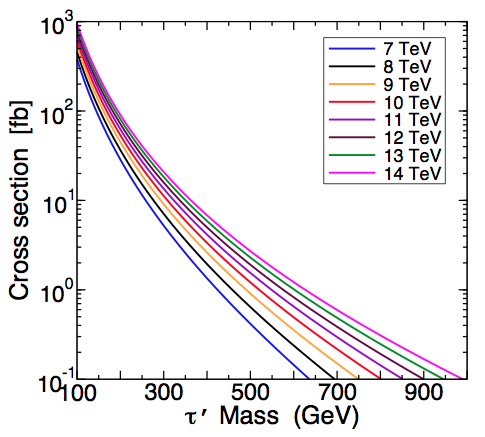
\includegraphics{figures/ch7-resonance/vll_xsec.png}}
  \caption{Cross sections for $pp\rightarrow \lpm\lmp$ for the vector-like leptons model, from~\cite{Martin:2012dg}. The $\tau'$ in the figure is the heavy fermion $\lpm$ in this analysis.}
  \label{fig:vll-xsec}
\end{figure}

\section{Search Strategy}
\subsection{Event Selection and Heavy Lepton Reconstruction}\label{sec:event-3l-selection}
Events containing a heavy lepton candidate are selected as follows:
\begin{itemize}
	\item Require a primary vertex with at least three tracks with $\pt>400~\mbox{MeV}$.
	\item Require at least three electrons or muons ($eee$, $ee\mu$, $\mu\mu e$, $\mu\mu\mu$) satisfying the lepton cuts (table~\ref{table:lepton-selections}). 
	\item Require a $Z$ candidate, consisting of a same-flavor, opposite-sign pair of leptons with $|m_{l^+l^-}-m_{Z}|<10~\mbox{GeV}$. The $Z$ mass is taken to be $91.1876~\mbox{GeV}$~\cite{PhysRevD.86.010001}. 
	\item Four-lepton events with two leptonic $Z$ candidates are rejected to suppresses background from $ZZ$ events. The efficiency loss for signal events is low, in part due to the additional factor of the leptonic branching ratio of the $Z$; see tables~\ref{table:fiducial-efficiencies-Ze} and \ref{table:fiducial-efficiencies-Zmu}. 
	\item Choose a unique trilepton candidate in each event as follows:
	\begin{itemize}
		\item Choose the same-flavor, opposite-sign (SFOS) pair with invariant mass closest to $m_{Z}$.
		\item Choose the third (``bachelor'') lepton to be the closest in $\Delta R$ to the reconstructed $Z$ four-momentum.
	\end{itemize}
  \item For low heavy lepton mass hypotheses, $m_{\lpm}\lesssim 200~\mbox{GeV}$, the $Z$ and the third lepton will tend to be collimated. This is shown qualitatively in a scatter plot of $\deltam=m_{3l}-m_{l^+l^-}$~\footnote{The invariant mass of the same-flavor, opposite-sign pair is subtracted from the trilepton mass in order to cancel some of the mass resolution due to the two leptons from the on-shell $Z$.} vs. $\Delta R(Z,\ l_3)$ in figure~\ref{fig:DeltaM-dR}. The expected background and signal $\Delta R$ distributions in the inclusive signal region are shown in figure~\ref{fig:inclusive-SR-dR}. A cut on $\Delta R(Z,\ l_3)$ helps to refine the signal, and also provides a useful control region by inverting the cut.

  \begin{figure}[h]
  	\centering
  	\resizebox{0.6\textwidth}{!}{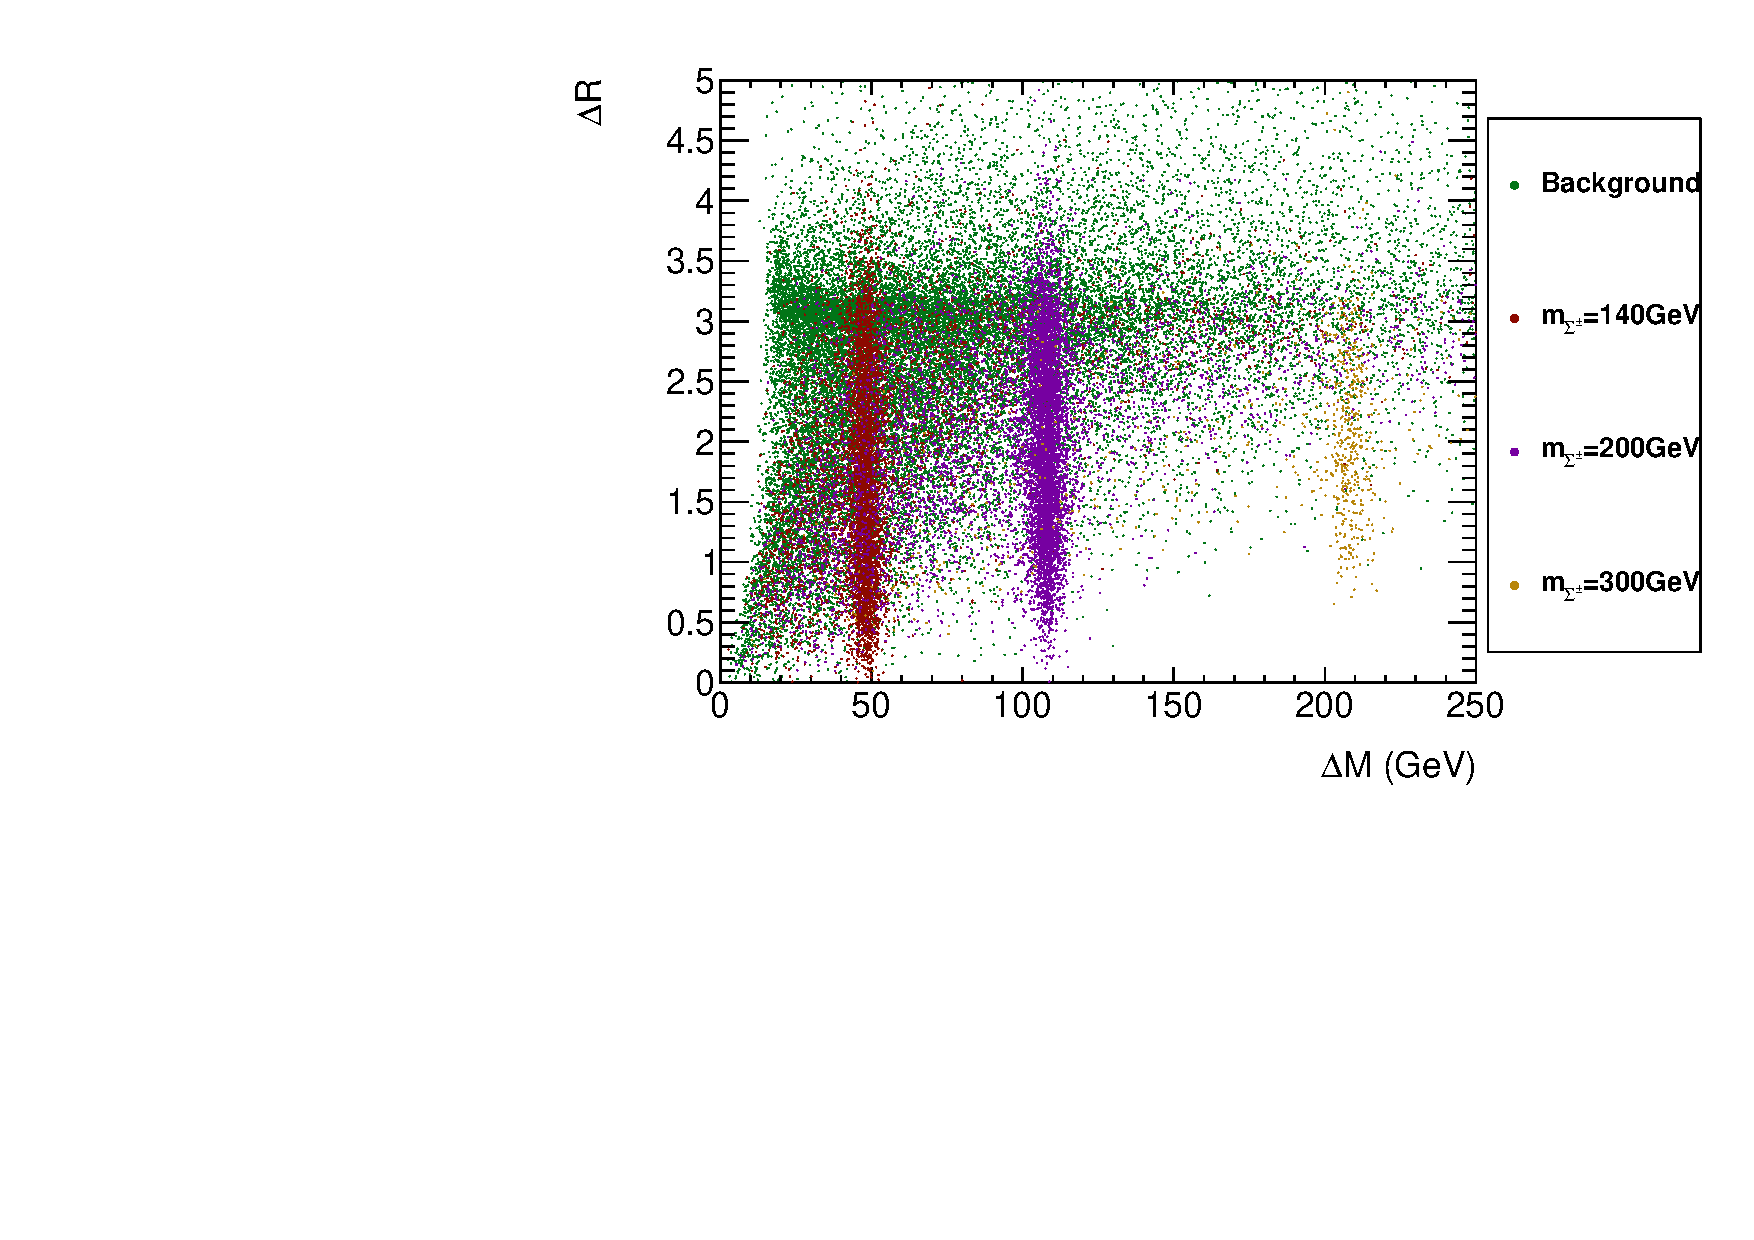
\includegraphics{figures/ch7-resonance/c_DeltaM_vs_DeltaR_Ze}}
  	\caption{Scatter plot of $\deltam$ vs. $\Delta R(Z,\ l_3)$ for signal and background events in the inclusive $Z+e$ signal region.}
  	\label{fig:DeltaM-dR}
  \end{figure}

 \begin{figure}[h]
 	\centering
 	\resizebox{0.6\textwidth}{!}{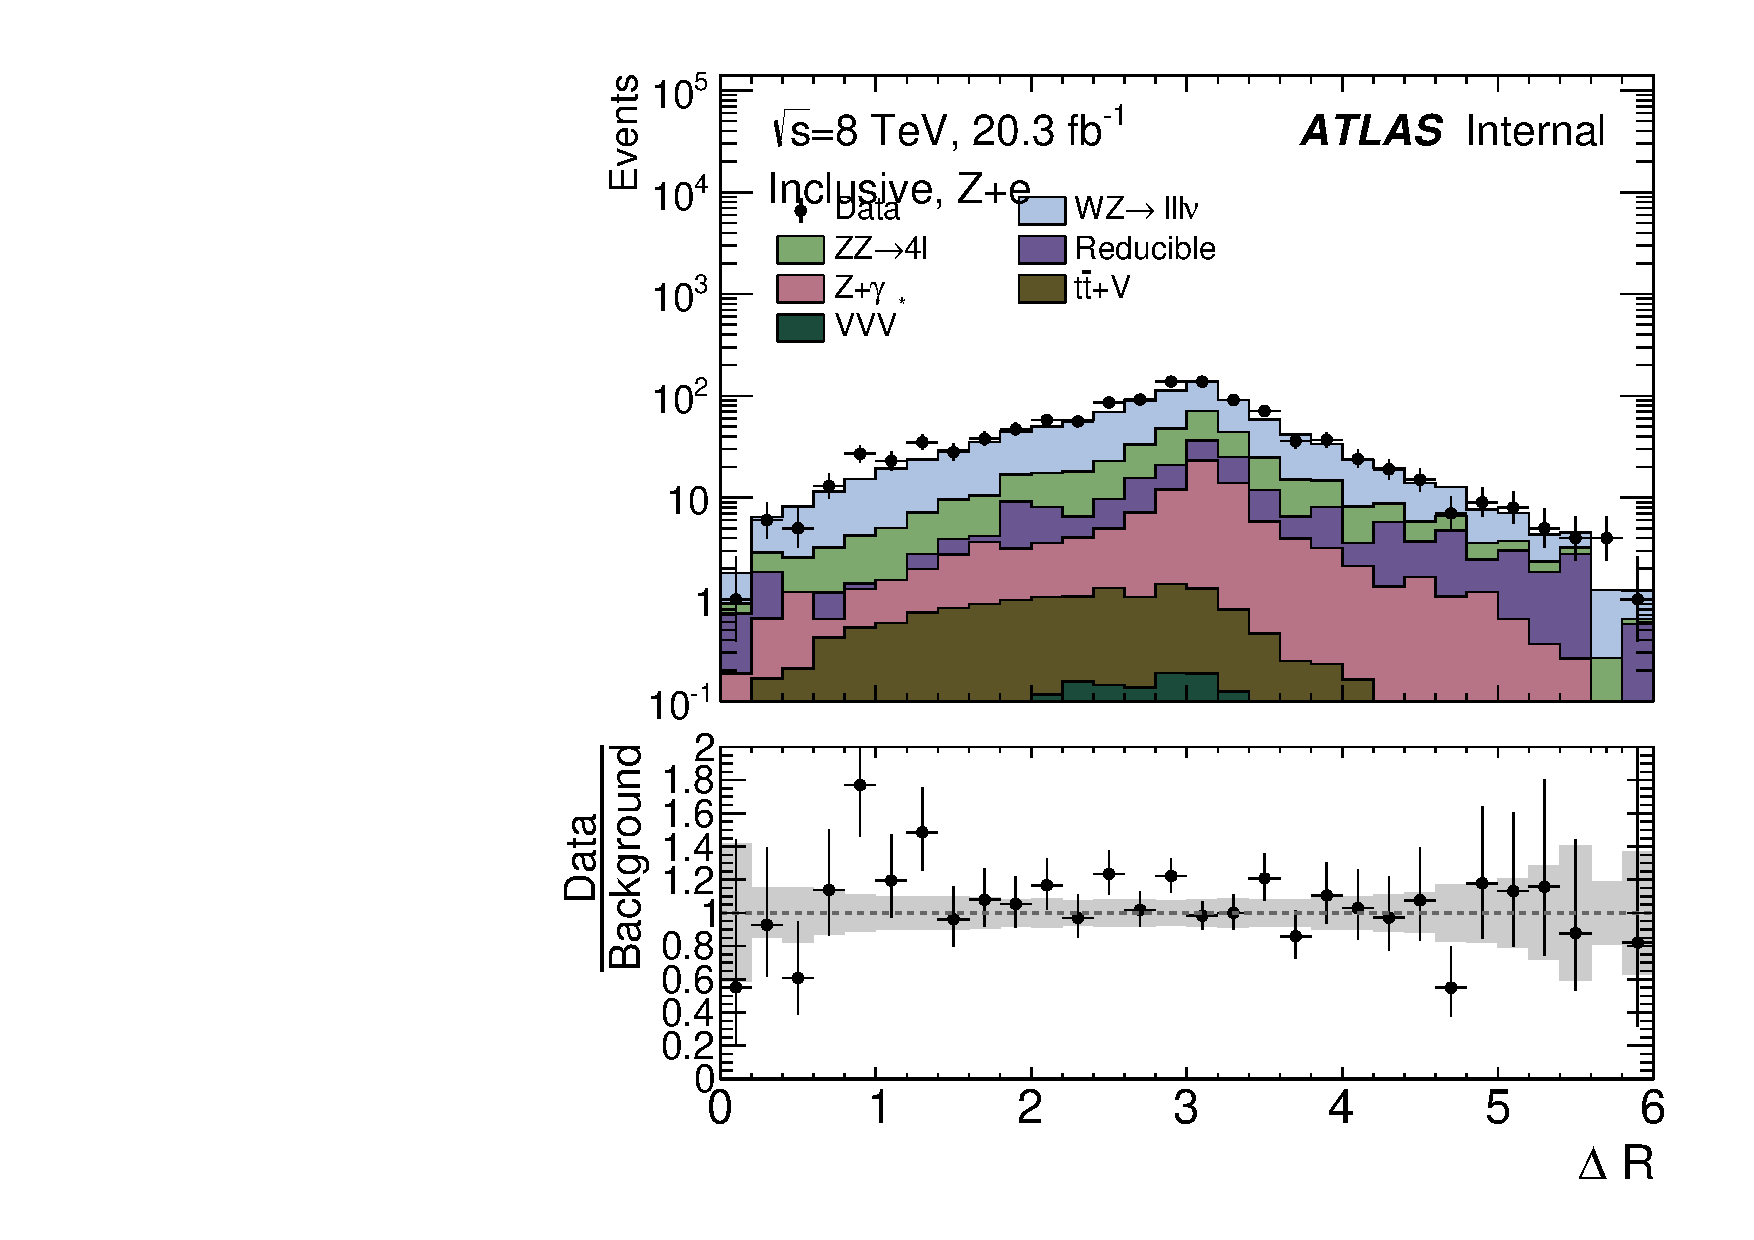
\includegraphics{figures/ch7-resonance/c_output_dR_Ze_InclusiveNoM3LDeltaR_300GeV_log}}
 	\caption{Expected $\Delta R(Z,\ l_3)$ distributions for background and signal in the inclusive signal region.}
 	\label{fig:inclusive-SR-dR}
 \end{figure}
  
  The cut on $\Delta R(Z,\ l_3)$ is chosen by running the cut-and-count based limit setting, described in section~\ref{sec:limit-method-mass-windows}, with different values of the $\Delta R$ cut. For cut values of $\Delta R < 2.0,\ 2.25,\ 2.5,\ 2.75,\ 3.0,\ 3.14,\ 3.5,$ and $4.0$, the expected exclusions were determined using \verb.mclimits., based on the expected signal and background yields in narrow mass windows around the signal mass hypotheses. For simplicity, the same $\Delta R(Z,\ l_3)$ cut is applied to all categories; no significant gain is observed by optimizing each category individually. The expected exclusions for different $\Delta R(Z,\ l_3)$ cuts are shown in figure~\ref{fig:dR-optimization}. Smaller values of the cut ($\Delta R(Z,\ l_3)\lesssim 2.0$) perform similarly to more stringent cuts at low signal mass hypotheses, but decline at higher mass hypotheses. Cuts above $\Delta R(Z,\ l_3)\lesssim 3.0$ perform approximately equally. Based on these studies, and also to use the inverse of this cut to define a control region, a cut value of $\Delta R(Z,\ l_3)<3.0$ is chosen. 

  \begin{figure}[h]
  	\subfloat[Vector-Like Leptons] {
  		\resizebox{0.45\textwidth}{!}{\includegraphics{figures/ch7-resonance/{c_limits_dRVariation_VLL_Combined_BRe1.0_BRmu0.0}.pdf}}
  	}
  	\subfloat[Seesaw] {
  		\resizebox{0.45\textwidth}{!}{\includegraphics{figures/ch7-resonance/{c_limits_dRVariation_Seesaw_Combined_BRe1.0_BRmu0.0}.pdf}}
  	}
  	\caption{Expected upper limits on cross section times branching ratio to final states with least one trilepton resonant decay for different cuts on $\Delta R(Z,\ l_3)$.}
  	\label{fig:dR-optimization}
  \end{figure}
  

  \item Six mutually exclusive signal regions are defined. Events are divided into two flavor channels, $Z+e$ and $Z+\mu$, depending on the flavor the bachelor lepton, and into three exclusive categories based on other activity in the event:
  \begin{itemize}
  	\item \textbf{\fourl}: Event contains a fourth lepton, either an electron or a muon, passing the normal lepton criteria. 
  	\item \textbf{\threeljj}: Event contains exactly three leptons, and a dijet with $60.385~\mbox{GeV}<m_{jj}<150.9~\mbox{GeV}$. 
  	\item \textbf{\threelo}: All other events, i.e. events with three leptons and no jet pair satisying the invariant mass requirement. 
  \end{itemize}
\end{itemize}

 The division into the three signal regions targeting the opposite side decay is motivated in figure~\ref{fig:opposite-side-br}, which shows the fraction of events with various activity from the decay of the other heavy lepton. The decays mostly contain extra leptons and neutrinos, and jets from $W/Z/h$ decays. Three categories are defined to take advantage of the additional activity, defined by requiring a fourth lepton, a high-mass dijet ($m_{W}-20~\mbox{GeV}<m_{jj}<m_{h}+25~\mbox{GeV}$), and everything else. The dijet mass window was not optimized, but was simply chosen to be widely inclusive of dijet boson decays. At truth level, the requirement of either a fourth lepton or a hadronically decaying boson is very efficient on signal: if the second heavy fermion is charged, then every decay satisfies this requirement, while if the second heavy fermion is neutral, then every decay except for $\Sigma^0\rightarrow Z\nu\rightarrow \nu\nu\nu$ and low branching fraction Higgs decays satisfies this requirement. Further, categorization targeting neutrinos is less effective at separating signal from the large $WZ$ background (see figures~\ref{fig:SR-mTW-1}-\ref{fig:SR-ETMiss-2}). 

In some cases, it is useful to consider the events without dividing into these three categories, but rather only the flavor of the bachelor lepton. This is referred to as the ``Inclusive'' signal region below.

\begin{figure}
	\subfloat[ $\lpm$] {
		\resizebox{0.48\textwidth}{!}{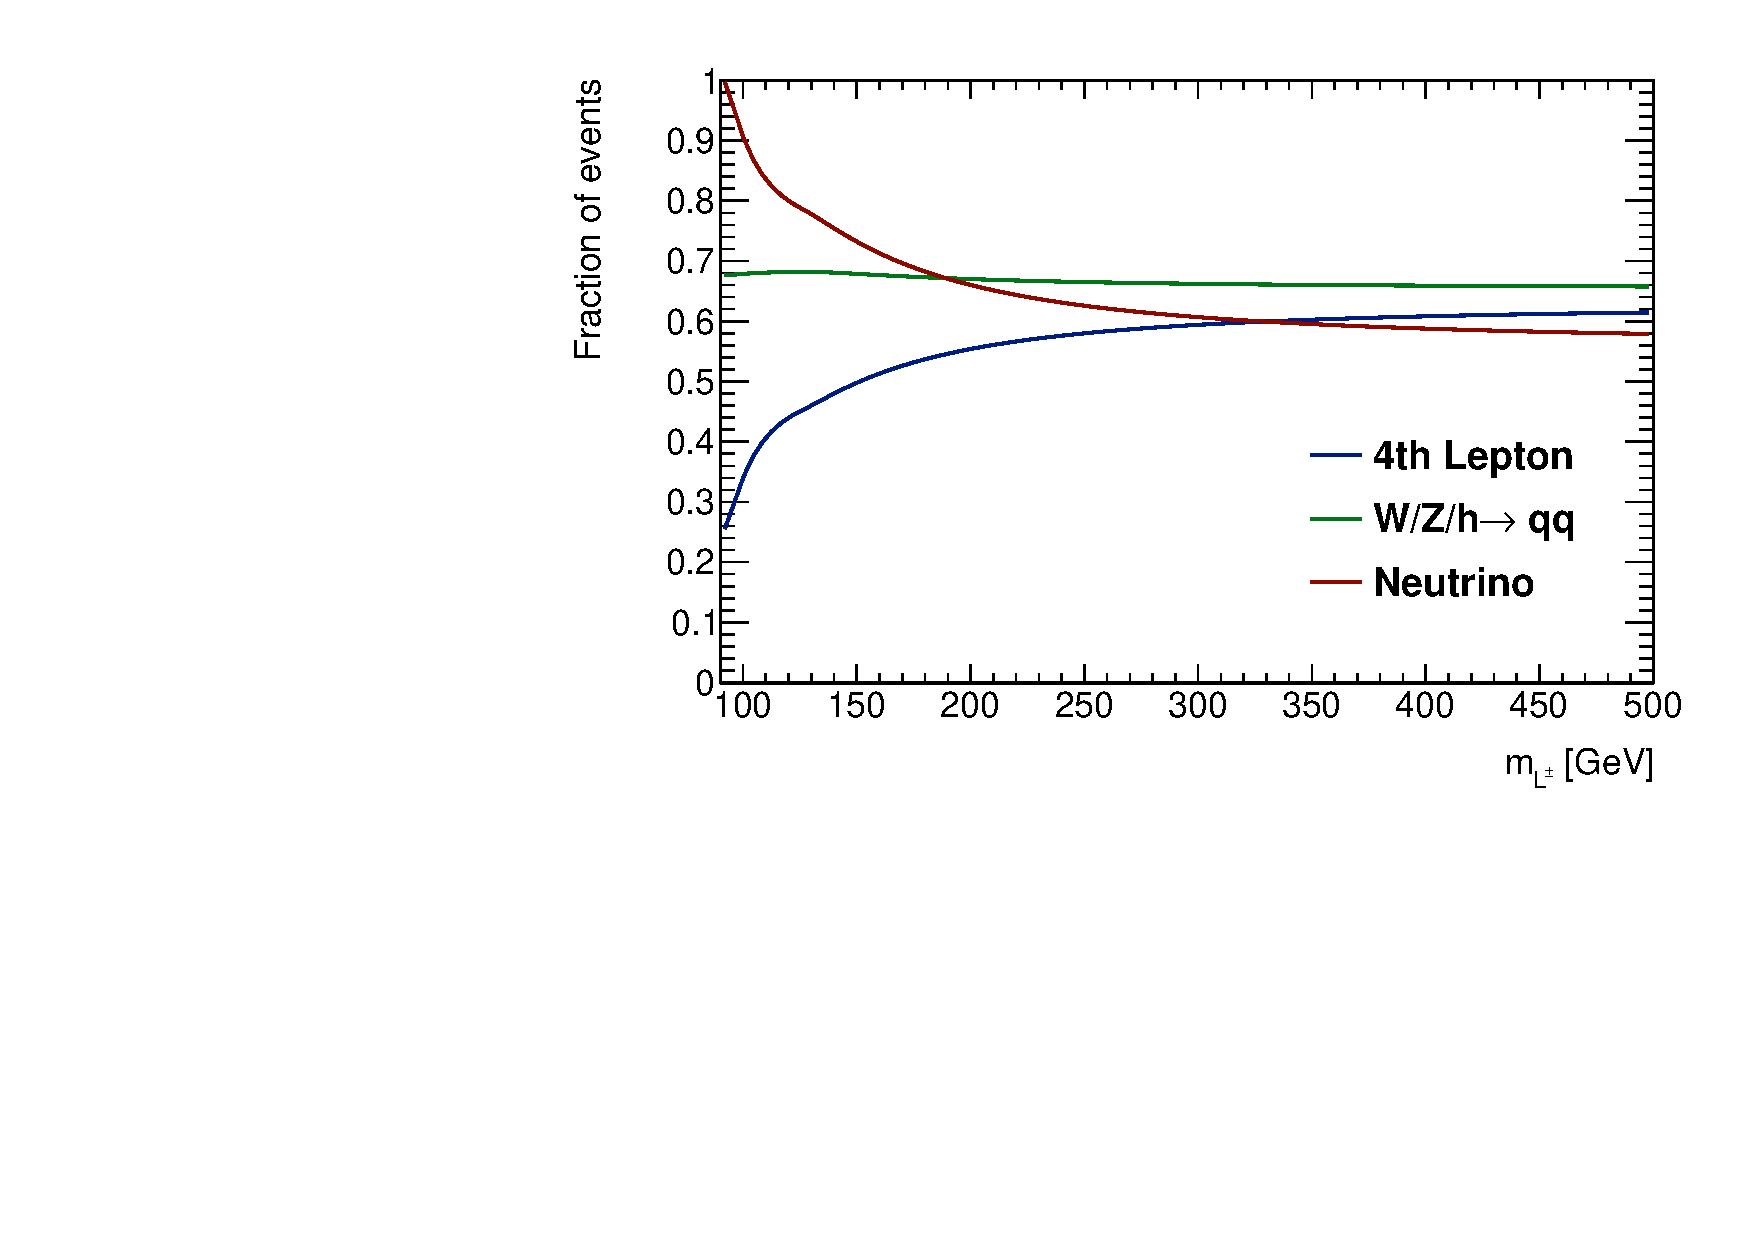
\includegraphics{figures/ch7-resonance/c_oppositeside_charged.pdf}}
	}
	\subfloat[ $\lzero$] {
		\resizebox{0.48\textwidth}{!}{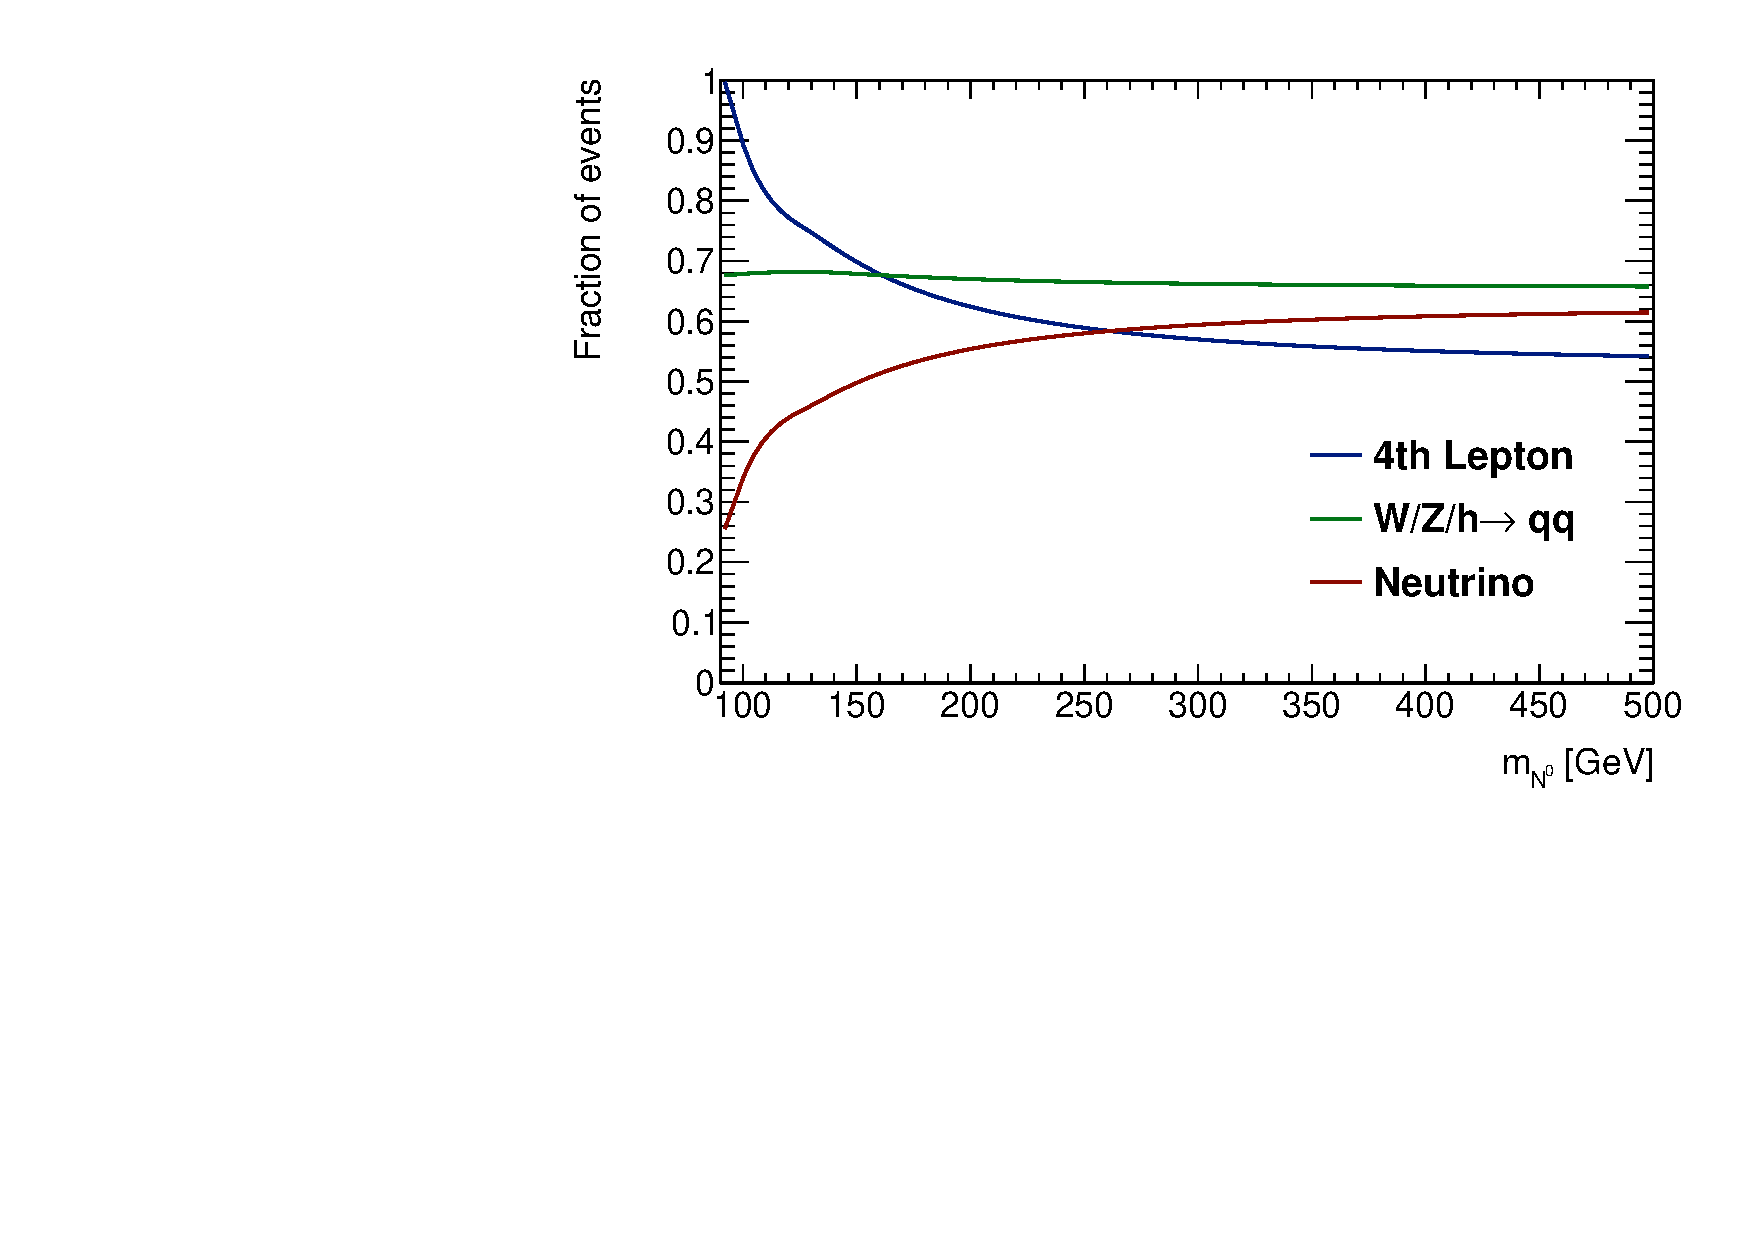
\includegraphics{figures/ch7-resonance/c_oppositeside_neutral.pdf}}
	}
	\caption{Fraction of events with various activity on the opposite side of the event, for $\lpm\Sigma^{\mp}$ events at left, and $\lpm\Sigma^0$ events at right. The left plot, showing the opposite side activity for a $\lpm\Sigma^{\mp}$ final state, is identical for the seesaw and vector-like lepton model.
	}
	\label{fig:opposite-side-br}
\end{figure}

\subsection{Performance on Fiducial Signal Events}\label{sec:fiducial-cutflow}
The performance of the cuts and heavy lepton candidate selection is shown in tables~\ref{table:fiducial-efficiencies-Ze} and \ref{table:fiducial-efficiencies-Zmu} in terms of efficiency on fiducial events. The final efficiency for each signal region is shown as a function of signal mass $m_{\Sigma}$ in figure~\ref{fig:fiducial-efficiencies-vs-mass}. The study is performed separately for the $Z+e$ and $Z+\mu$ flavor channels. The fiducial selection requires the event to have three truth-level leptons satisfying $\pt>15~\mbox{GeV}$ and $|\eta|<2.5$, of which two form a $Z$ candidate with $|m_{l^+l^-}-m_Z|<10~\mbox{GeV}$, the third lepton is of the correct flavor, and the trilepton mass satisfies $|m_{3l}-m_{\lpm}|<5~\mbox{GeV}$.

Note that cut imposing a flavor requirement on the reconstructed bachelor lepton has a different efficiency between the vector-like lepton sample and the seeaw sample. This is a consequence of the initial flavor content of the samples: the vector-like lepton samples are divided into two samples with with 100\% branching fraction to either bachelor electron or bachelor muon, while the seesaw samples is a single mixed sample containing both electron and muon decays. 


\begin{table}[ht]
	\resizebox{\textwidth}{!}{
	\begin{tabular}{|c|c|c|c|c|c||c|c|c|}
		\hline
		Process  & Preselection  & Bachelor $e$  & $|m_{l^{+}l^{-}} - m_{Z}|<10~\mbox{GeV}$  & !$2Z$  & $\Delta R < 3.0$  & $4l$ & $3l+jj$ & Else \\
		\hline
		VLL, $100$~GeV		&	$0.348 \pm 0.008$	&	$0.318 \pm 0.008$	&	$0.306 \pm 0.008$	&	$0.303 \pm 0.008$	&	$0.298 \pm 0.008$	&	$0.054 \pm 0.004$ &	$0.096 \pm 0.005$	&	$0.147 \pm 0.006$	\\
		\hline
		VLL, $110$~GeV		&	$0.478 \pm 0.006$	&	$0.435 \pm 0.006$	&	$0.421 \pm 0.006$	&	$0.417 \pm 0.006$	&	$0.401 \pm 0.006$	&	$0.076 \pm 0.003$ &	$0.11 \pm 0.004$	&	$0.215 \pm 0.005$	\\
		\hline
		VLL, $120$~GeV		&	$0.535 \pm 0.006$	&	$0.491 \pm 0.006$	&	$0.467 \pm 0.006$	&	$0.457 \pm 0.006$	&	$0.424 \pm 0.006$	&	$0.104 \pm 0.004$ &	$0.117 \pm 0.004$	&	$0.204 \pm 0.005$	\\
		\hline
		VLL, $130$~GeV		&	$0.604 \pm 0.006$	&	$0.539 \pm 0.006$	&	$0.509 \pm 0.006$	&	$0.494 \pm 0.006$	&	$0.445 \pm 0.006$	&	$0.125 \pm 0.004$ &	$0.127 \pm 0.004$	&	$0.194 \pm 0.005$	\\
		\hline
		VLL, $140$~GeV		&	$0.643 \pm 0.006$	&	$0.578 \pm 0.006$	&	$0.559 \pm 0.006$	&	$0.538 \pm 0.006$	&	$0.491 \pm 0.006$	&	$0.153 \pm 0.004$ &	$0.164 \pm 0.004$	&	$0.174 \pm 0.005$	\\
		\hline
		VLL, $160$~GeV		&	$0.663 \pm 0.006$	&	$0.593 \pm 0.006$	&	$0.572 \pm 0.006$	&	$0.552 \pm 0.006$	&	$0.499 \pm 0.006$	&	$0.175 \pm 0.005$ &	$0.148 \pm 0.004$	&	$0.176 \pm 0.005$	\\
		\hline
		VLL, $180$~GeV		&	$0.698 \pm 0.006$	&	$0.62 \pm 0.006$	&	$0.594 \pm 0.006$	&	$0.573 \pm 0.007$	&	$0.505 \pm 0.007$	&	$0.197 \pm 0.005$ &	$0.163 \pm 0.005$	&	$0.144 \pm 0.005$	\\
		\hline
		VLL, $200$~GeV		&	$0.707 \pm 0.006$	&	$0.624 \pm 0.007$	&	$0.596 \pm 0.007$	&	$0.577 \pm 0.007$	&	$0.52 \pm 0.007$	&	$0.209 \pm 0.006$ &	$0.167 \pm 0.005$	&	$0.145 \pm 0.005$	\\
		\hline
		VLL, $250$~GeV		&	$0.751 \pm 0.007$	&	$0.654 \pm 0.007$	&	$0.626 \pm 0.007$	&	$0.615 \pm 0.007$	&	$0.548 \pm 0.008$	&	$0.245 \pm 0.007$ &	$0.152 \pm 0.005$	&	$0.151 \pm 0.005$	\\
		\hline
		VLL, $300$~GeV		&	$0.771 \pm 0.007$	&	$0.662 \pm 0.008$	&	$0.63 \pm 0.008$	&	$0.625 \pm 0.008$	&	$0.547 \pm 0.008$	&	$0.258 \pm 0.007$ &	$0.169 \pm 0.006$	&	$0.121 \pm 0.005$	\\
		\hline
		VLL, $400$~GeV		&	$0.776 \pm 0.007$	&	$0.669 \pm 0.008$	&	$0.642 \pm 0.008$	&	$0.641 \pm 0.008$	&	$0.562 \pm 0.008$	&	$0.277 \pm 0.007$ &	$0.181 \pm 0.006$	&	$0.103 \pm 0.005$	\\
		\hline
		Seesaw, $100$~GeV	&	$0.381 \pm 0.006$	&	$0.351 \pm 0.005$	&	$0.336 \pm 0.005$	&	$0.334 \pm 0.005$	&	$0.308 \pm 0.005$	&	$0.08 \pm 0.003$ &	$0.096 \pm 0.003$	&	$0.131 \pm 0.004$	\\
		\hline
		Seesaw, $120$~GeV	&	$0.517 \pm 0.004$	&	$0.474 \pm 0.004$	&	$0.45 \pm 0.004$	&	$0.44 \pm 0.004$	&	$0.403 \pm 0.004$	&	$0.128 \pm 0.003$ &	$0.128 \pm 0.003$	&	$0.148 \pm 0.003$	\\
		\hline
		Seesaw, $160$~GeV	&	$0.611 \pm 0.005$	&	$0.548 \pm 0.005$	&	$0.532 \pm 0.005$	&	$0.516 \pm 0.005$	&	$0.464 \pm 0.005$	&	$0.167 \pm 0.004$ &	$0.141 \pm 0.003$	&	$0.157 \pm 0.003$	\\
		\hline
		Seesaw, $200$~GeV	&	$0.657 \pm 0.005$	&	$0.591 \pm 0.005$	&	$0.574 \pm 0.005$	&	$0.559 \pm 0.005$	&	$0.5 \pm 0.005$		&	$0.203 \pm 0.004$ &	$0.146 \pm 0.003$	&	$0.152 \pm 0.004$	\\
		\hline
		Seesaw, $250$~GeV	&	$0.671 \pm 0.007$	&	$0.605 \pm 0.007$	&	$0.592 \pm 0.007$	&	$0.582 \pm 0.007$	&	$0.505 \pm 0.007$	&	$0.221 \pm 0.006$ &	$0.14 \pm 0.005$	&	$0.144 \pm 0.005$	\\
		\hline
		Seesaw, $300$~GeV	&	$0.729 \pm 0.007$	&	$0.649 \pm 0.007$	&	$0.633 \pm 0.007$	&	$0.626 \pm 0.007$	&	$0.541 \pm 0.008$	&	$0.23 \pm 0.006$ &	$0.167 \pm 0.006$	&	$0.144 \pm 0.005$	\\
		\hline
		Seesaw, $350$~GeV	&	$0.72 \pm 0.007$	&	$0.651 \pm 0.008$	&	$0.638 \pm 0.008$	&	$0.635 \pm 0.008$	&	$0.553 \pm 0.008$	&	$0.251 \pm 0.007$ &	$0.157 \pm 0.006$	&	$0.146 \pm 0.006$	\\
		\hline
		Seesaw, $400$~GeV	&	$0.717 \pm 0.007$	&	$0.641 \pm 0.008$	&	$0.627 \pm 0.008$	&	$0.623 \pm 0.008$	&	$0.529 \pm 0.008$	&	$0.243 \pm 0.007$ &	$0.15 \pm 0.006$	&	$0.136 \pm 0.005$	\\
		\hline
		Seesaw, $450$~GeV	&	$0.762 \pm 0.008$	&	$0.67 \pm 0.009$	&	$0.66 \pm 0.009$	&	$0.657 \pm 0.009$	&	$0.554 \pm 0.009$	&	$0.267 \pm 0.008$ &	$0.184 \pm 0.007$	&	$0.103 \pm 0.006$	\\
		\hline
		Seesaw, $500$~GeV	&	$0.72 \pm 0.007$	&	$0.636 \pm 0.008$	&	$0.611 \pm 0.008$	&	$0.608 \pm 0.008$	&	$0.525 \pm 0.008$	&	$0.24 \pm 0.007$ &	$0.151 \pm 0.006$	&	$0.134 \pm 0.005$	\\
		\hline
	\end{tabular}
	}
	\caption{Cut efficiencies for fiducial events at various stages in the cutflow for the $Z+e$ signal regions. Only statistical uncertainties due to finite Monte Carlo statistics are shown. The preselection cut requires three selected leptons, with one same-flavor opposite-sign pair, as well as the general event selection cuts listed above.}
	\label{table:fiducial-efficiencies-Ze}
\end{table}

\begin{table}[ht]
	\resizebox{\textwidth}{!}{
	\begin{tabular}{|c|c|c|c|c|c||c|c|c|}
		\hline
		Process  & Preselection  & Bachelor $\mu$  & $|m_{l^{+}l^{-}} - m_{Z}|<10~\mbox{GeV}$  & !$2Z$  & $\Delta R < 3.0$  & $4l$ & $3l+jj$ & Else \\
		\hline
		VLL, $100$~GeV	&	$0.52 \pm 0.007$	&	$0.508 \pm 0.007$	&	$0.472 \pm 0.007$	&	$0.461 \pm 0.007$	&	$0.456 \pm 0.007$	&	$0.064 \pm 0.004$ &	$0.14 \pm 0.005$	&	$0.252 \pm 0.006$\\
		\hline
		VLL, $110$~GeV	&	$0.61 \pm 0.004$	&	$0.593 \pm 0.004$	&	$0.568 \pm 0.004$	&	$0.554 \pm 0.004$	&	$0.536 \pm 0.004$	&	$0.119 \pm 0.003$ &	$0.142 \pm 0.003$	&	$0.275 \pm 0.004$\\
		\hline
		VLL, $120$~GeV	&	$0.67 \pm 0.003$	&	$0.648 \pm 0.004$	&	$0.617 \pm 0.004$	&	$0.596 \pm 0.004$	&	$0.561 \pm 0.004$	&	$0.149 \pm 0.003$ &	$0.139 \pm 0.003$	&	$0.273 \pm 0.003$\\
		\hline
		VLL, $130$~GeV	&	$0.702 \pm 0.003$	&	$0.676 \pm 0.003$	&	$0.642 \pm 0.003$	&	$0.614 \pm 0.003$	&	$0.569 \pm 0.003$	&	$0.163 \pm 0.003$ &	$0.143 \pm 0.002$	&	$0.263 \pm 0.003$\\
		\hline
		VLL, $140$~GeV	&	$0.723 \pm 0.003$	&	$0.701 \pm 0.003$	&	$0.667 \pm 0.003$	&	$0.634 \pm 0.003$	&	$0.585 \pm 0.003$	&	$0.173 \pm 0.003$ &	$0.156 \pm 0.002$	&	$0.256 \pm 0.003$\\
		\hline
		VLL, $160$~GeV	&	$0.752 \pm 0.003$	&	$0.727 \pm 0.003$	&	$0.685 \pm 0.003$	&	$0.65 \pm 0.003$	&	$0.592 \pm 0.003$	&	$0.212 \pm 0.003$ &	$0.156 \pm 0.002$	&	$0.223 \pm 0.003$\\
		\hline
		VLL, $180$~GeV	&	$0.77 \pm 0.003$	&	$0.746 \pm 0.003$	&	$0.69 \pm 0.003$	&	$0.659 \pm 0.003$	&	$0.593 \pm 0.003$	&	$0.227 \pm 0.003$ &	$0.161 \pm 0.002$	&	$0.205 \pm 0.003$\\
		\hline
		VLL, $200$~GeV	&	$0.779 \pm 0.003$	&	$0.751 \pm 0.003$	&	$0.69 \pm 0.003$	&	$0.66 \pm 0.003$	&	$0.584 \pm 0.003$	&	$0.239 \pm 0.003$ &	$0.161 \pm 0.002$	&	$0.184 \pm 0.002$\\
		\hline
		VLL, $250$~GeV	&	$0.786 \pm 0.003$	&	$0.752 \pm 0.003$	&	$0.676 \pm 0.003$	&	$0.657 \pm 0.003$	&	$0.579 \pm 0.003$	&	$0.268 \pm 0.003$ &	$0.162 \pm 0.002$	&	$0.149 \pm 0.002$\\
		\hline
		VLL, $300$~GeV	&	$0.789 \pm 0.002$	&	$0.76 \pm 0.003$	&	$0.68 \pm 0.003$	&	$0.667 \pm 0.003$	&	$0.578 \pm 0.003$	&	$0.288 \pm 0.003$ &	$0.163 \pm 0.002$	&	$0.127 \pm 0.002$\\
		\hline
		VLL, $400$~GeV	&	$0.787 \pm 0.002$	&	$0.753 \pm 0.003$	&	$0.665 \pm 0.003$	&	$0.656 \pm 0.003$	&	$0.563 \pm 0.003$	&	$0.292 \pm 0.003$ &	$0.166 \pm 0.002$	&	$0.106 \pm 0.002$\\
		\hline
		Seesaw, $100$~GeV	&	$0.535 \pm 0.006$	&	$0.521 \pm 0.006$	&	$0.484 \pm 0.006$	&	$0.471 \pm 0.006$	&	$0.46 \pm 0.006$	&	$0.192 \pm 0.005$ &	$0.121 \pm 0.004$	&	$0.147 \pm 0.004$\\
		\hline
		Seesaw, $120$~GeV	&	$0.677 \pm 0.004$	&	$0.66 \pm 0.004$	&	$0.613 \pm 0.004$	&	$0.589 \pm 0.004$	&	$0.546 \pm 0.004$	&	$0.212 \pm 0.004$ &	$0.119 \pm 0.003$	&	$0.215 \pm 0.004$\\
		\hline
		Seesaw, $160$~GeV	&	$0.745 \pm 0.004$	&	$0.723 \pm 0.004$	&	$0.685 \pm 0.004$	&	$0.658 \pm 0.004$	&	$0.595 \pm 0.005$	&	$0.252 \pm 0.004$ &	$0.14 \pm 0.003$	&	$0.202 \pm 0.004$\\
		\hline
		Seesaw, $200$~GeV	&	$0.743 \pm 0.004$	&	$0.717 \pm 0.005$	&	$0.668 \pm 0.005$	&	$0.651 \pm 0.005$	&	$0.588 \pm 0.005$	&	$0.263 \pm 0.004$ &	$0.152 \pm 0.004$	&	$0.173 \pm 0.004$\\
		\hline
		Seesaw, $250$~GeV	&	$0.761 \pm 0.006$	&	$0.735 \pm 0.006$	&	$0.673 \pm 0.007$	&	$0.662 \pm 0.007$	&	$0.585 \pm 0.007$	&	$0.284 \pm 0.006$ &	$0.144 \pm 0.005$	&	$0.157 \pm 0.005$\\
		\hline
		Seesaw, $300$~GeV	&	$0.785 \pm 0.006$	&	$0.764 \pm 0.006$	&	$0.695 \pm 0.007$	&	$0.688 \pm 0.007$	&	$0.601 \pm 0.007$	&	$0.295 \pm 0.007$ &	$0.171 \pm 0.006$	&	$0.135 \pm 0.005$\\
		\hline
		Seesaw, $350$~GeV	&	$0.78 \pm 0.006$	&	$0.757 \pm 0.007$	&	$0.688 \pm 0.007$	&	$0.681 \pm 0.007$	&	$0.59 \pm 0.008$	&	$0.294 \pm 0.007$ &	$0.155 \pm 0.006$	&	$0.141 \pm 0.005$\\
		\hline
		Seesaw, $400$~GeV	&	$0.753 \pm 0.007$	&	$0.727 \pm 0.007$	&	$0.642 \pm 0.008$	&	$0.634 \pm 0.008$	&	$0.544 \pm 0.008$	&	$0.277 \pm 0.007$ &	$0.15 \pm 0.006$	&	$0.118 \pm 0.005$\\
		\hline
		Seesaw, $450$~GeV	&	$0.762 \pm 0.008$	&	$0.732 \pm 0.008$	&	$0.658 \pm 0.008$	&	$0.653 \pm 0.009$	&	$0.555 \pm 0.009$	&	$0.285 \pm 0.008$ &	$0.152 \pm 0.006$	&	$0.119 \pm 0.006$\\
		\hline
		Seesaw, $500$~GeV	&	$0.755 \pm 0.007$	&	$0.729 \pm 0.007$	&	$0.654 \pm 0.008$	&	$0.65 \pm 0.008$	&	$0.551 \pm 0.008$	&	$0.275 \pm 0.007$ &	$0.155 \pm 0.006$	&	$0.122 \pm 0.005$\\
		\hline
	\end{tabular}
	}
	\caption{Cut efficiencies for fiducial events at various stages in the cutflow for the $Z+\mu$ signal regions. Only statistical uncertainties due to finite Monte Carlo statistics are shown. The preselection cut requires three selected leptons, with one same-flavor opposite-sign pair, as well as the general event selection cuts listed above.}
	\label{table:fiducial-efficiencies-Zmu}
\end{table}

\begin{figure}[htb]
	\centering
	\subfloat[ $Z+e$, seesaw] {
		\resizebox{0.4\textwidth}{!}{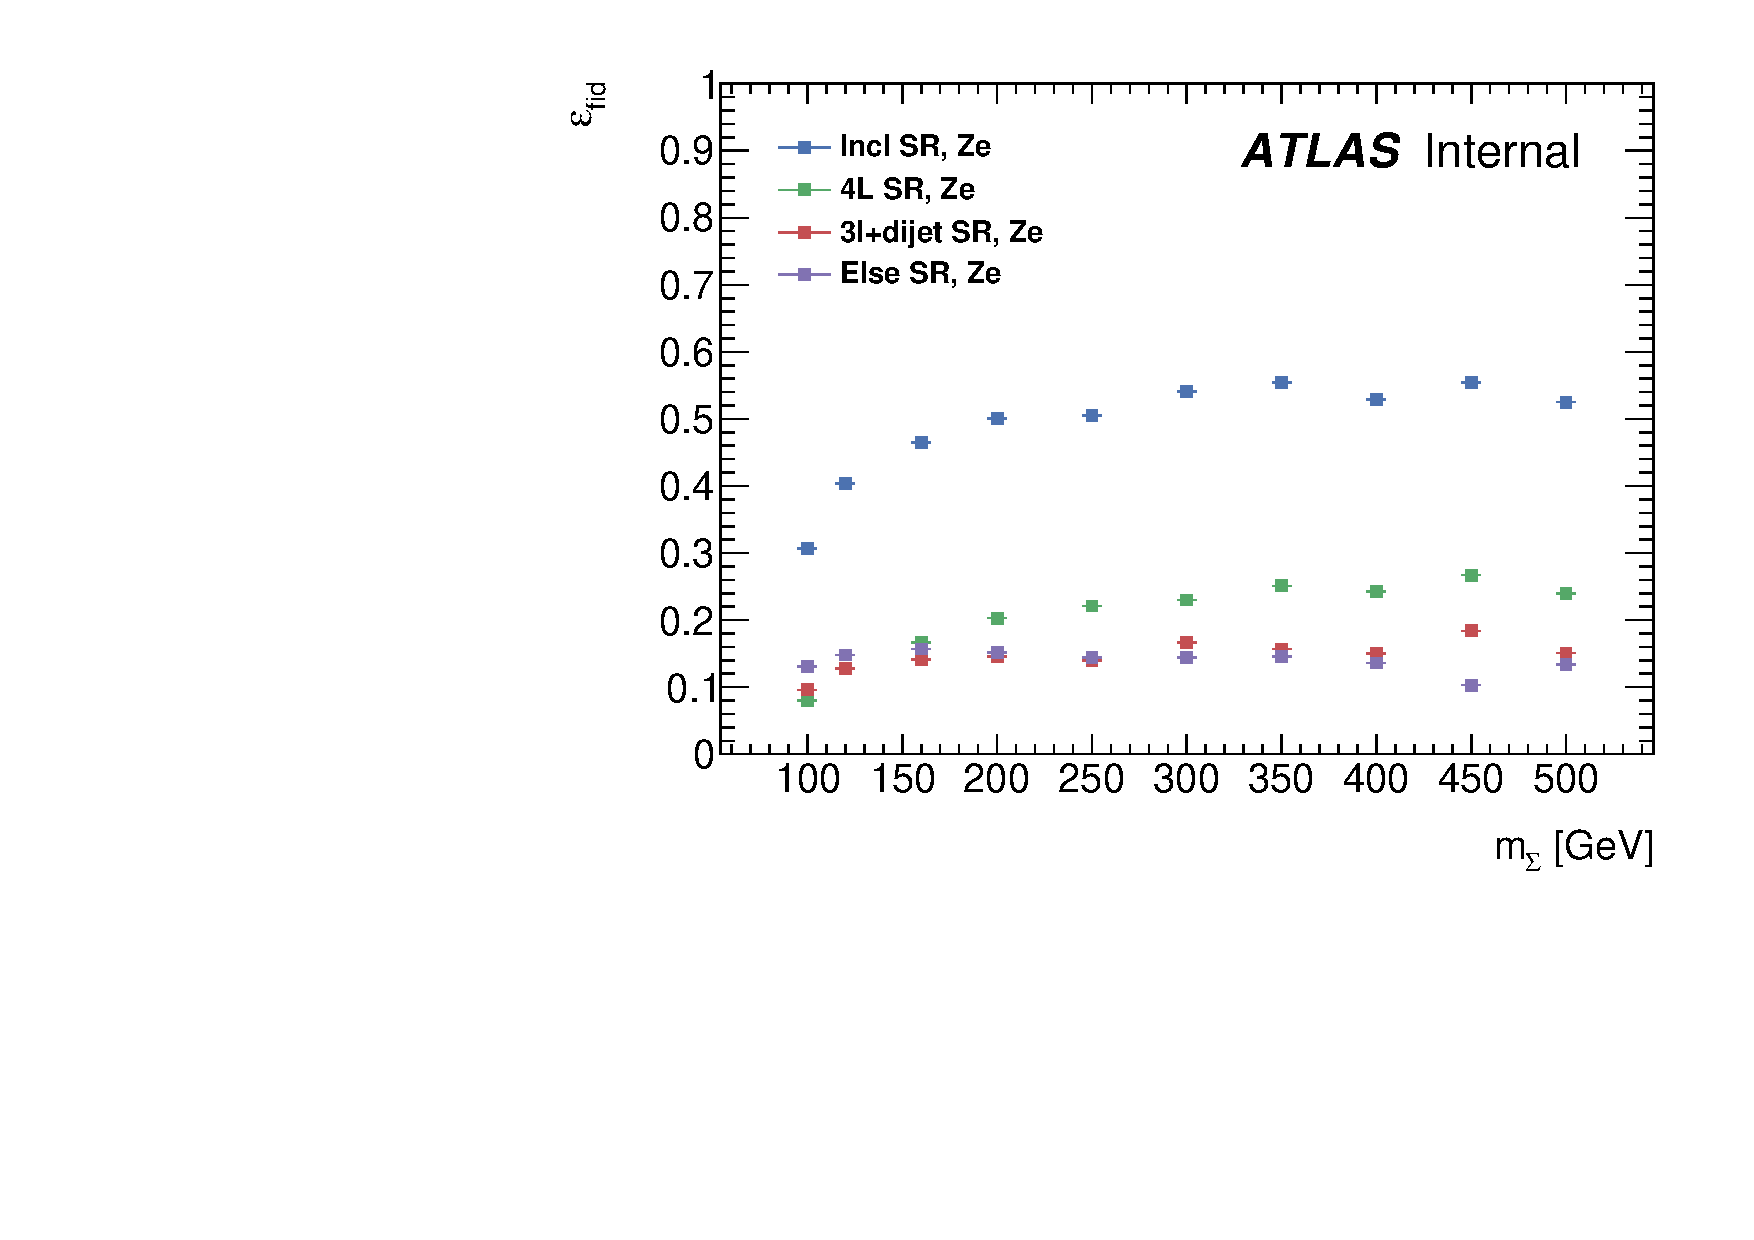
\includegraphics{figures/ch7-resonance/c_eff_fid_Ze_Seesaw}}
	}
	\subfloat[ $Z+e$, vector-like leptons] {
		\resizebox{0.4\textwidth}{!}{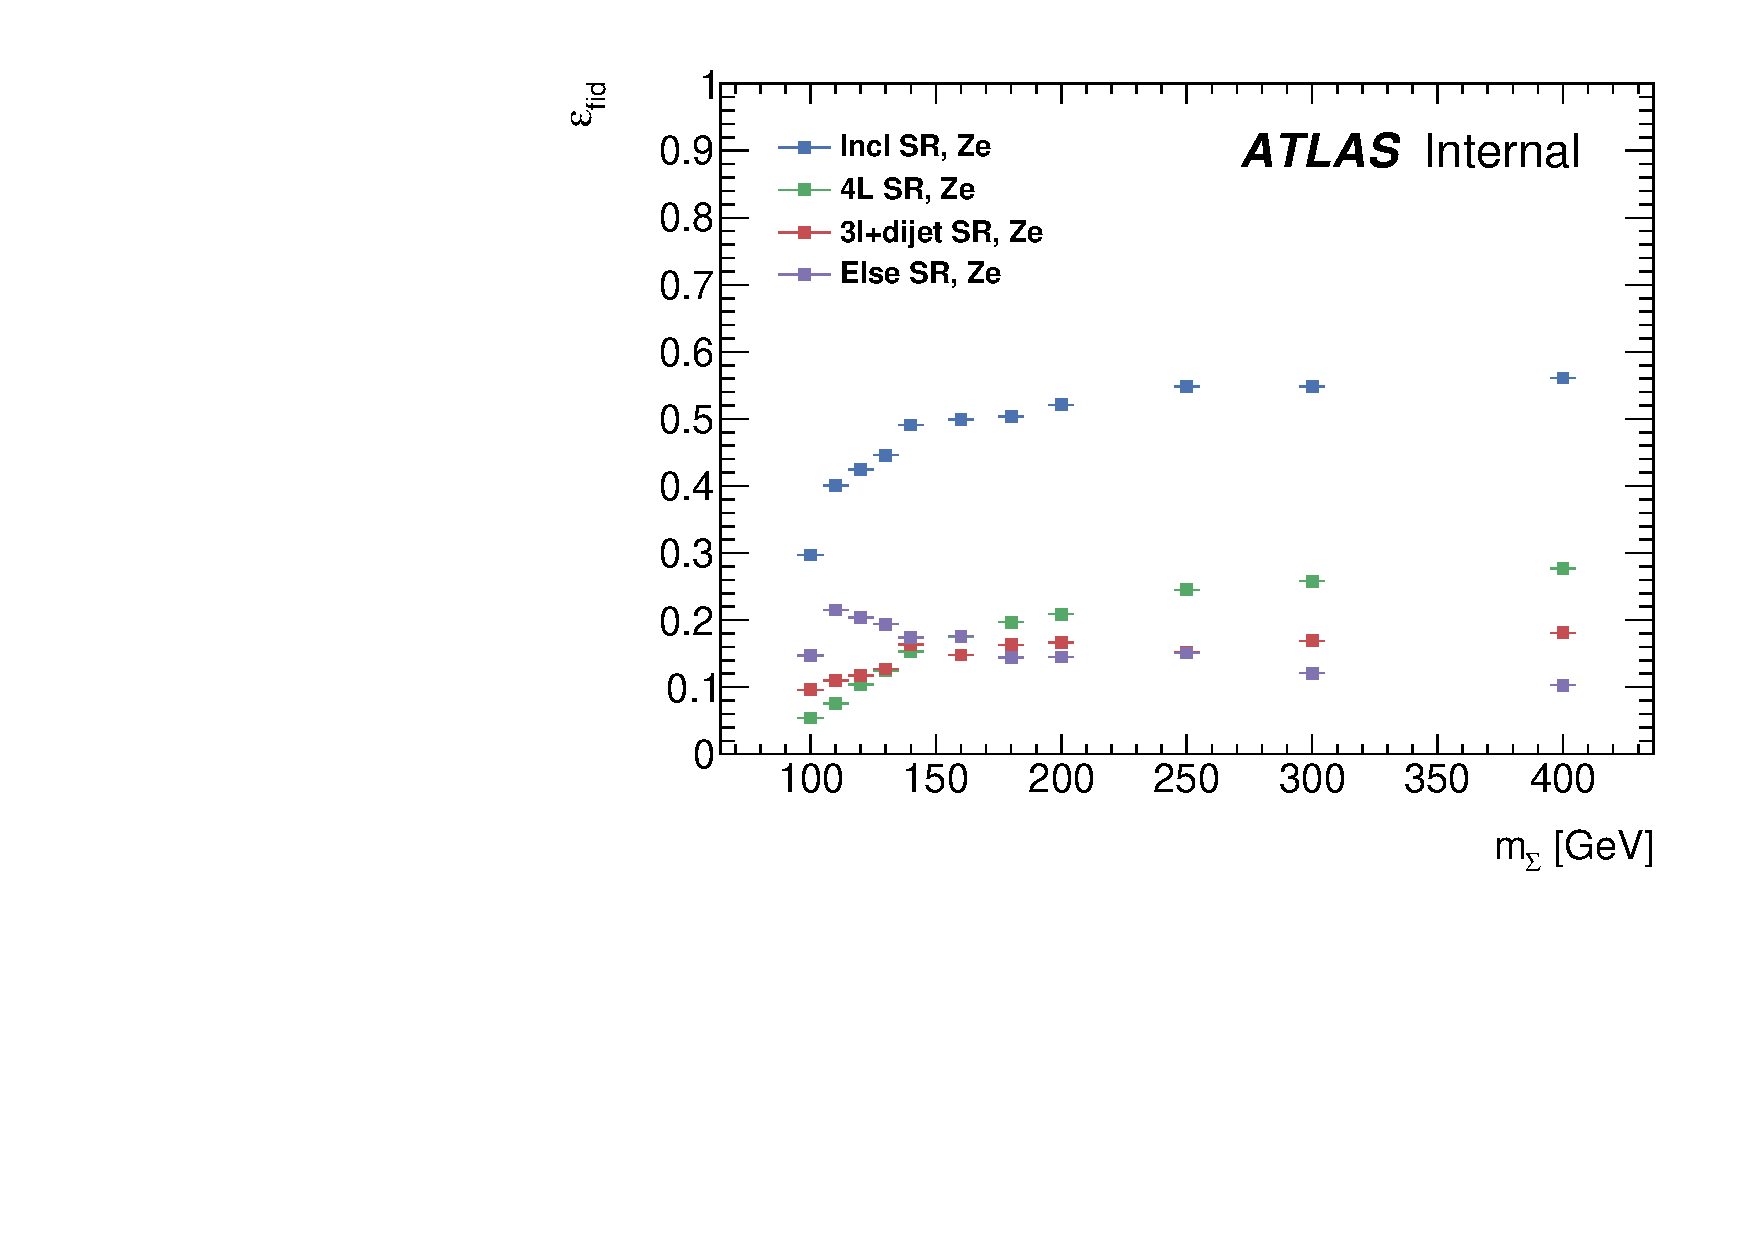
\includegraphics{figures/ch7-resonance/c_eff_fid_Ze_VLL}}
	} \\
	\subfloat[ $Z+\mu$, seesaw] {
		\resizebox{0.4\textwidth}{!}{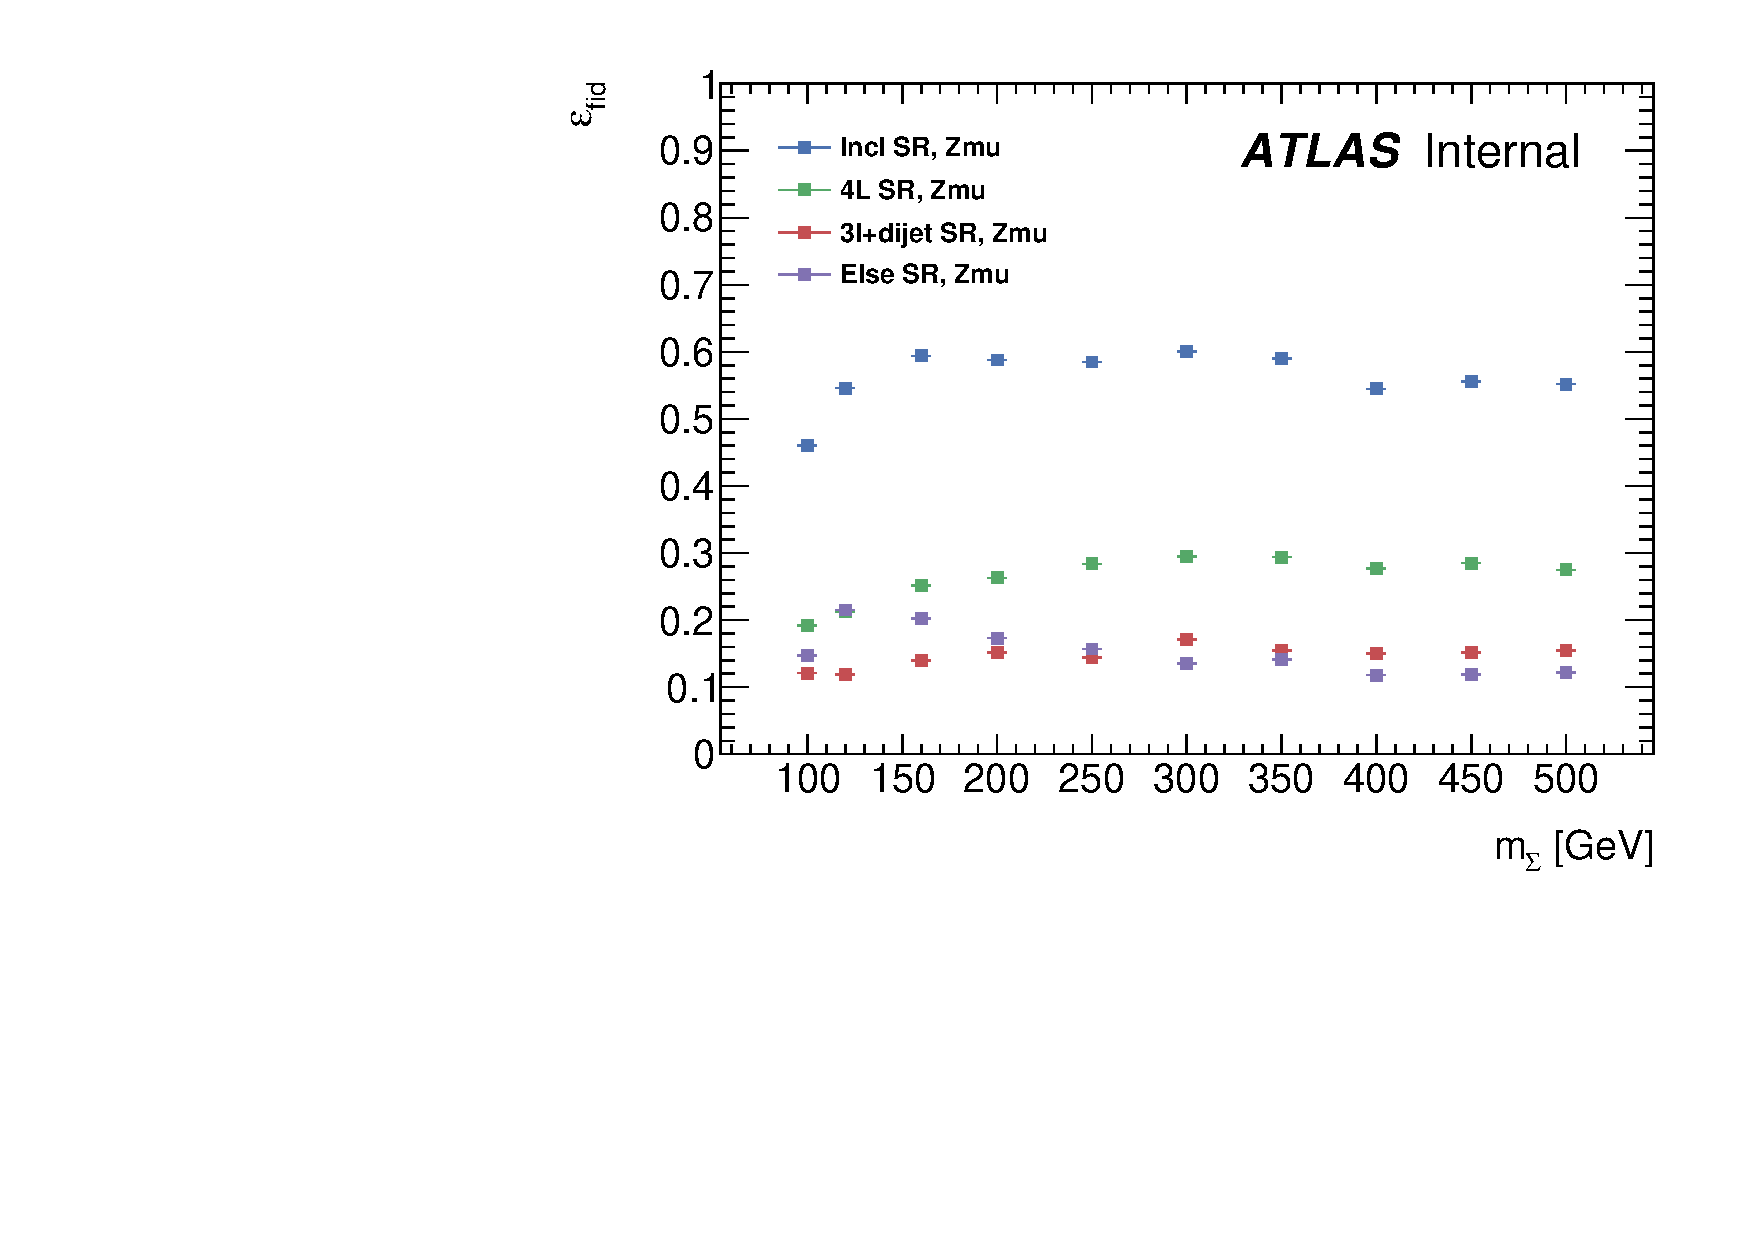
\includegraphics{figures/ch7-resonance/c_eff_fid_Zmu_Seesaw}}
	}
	\subfloat[ $Z+\mu$, vector-like leptons] {
		\resizebox{0.4\textwidth}{!}{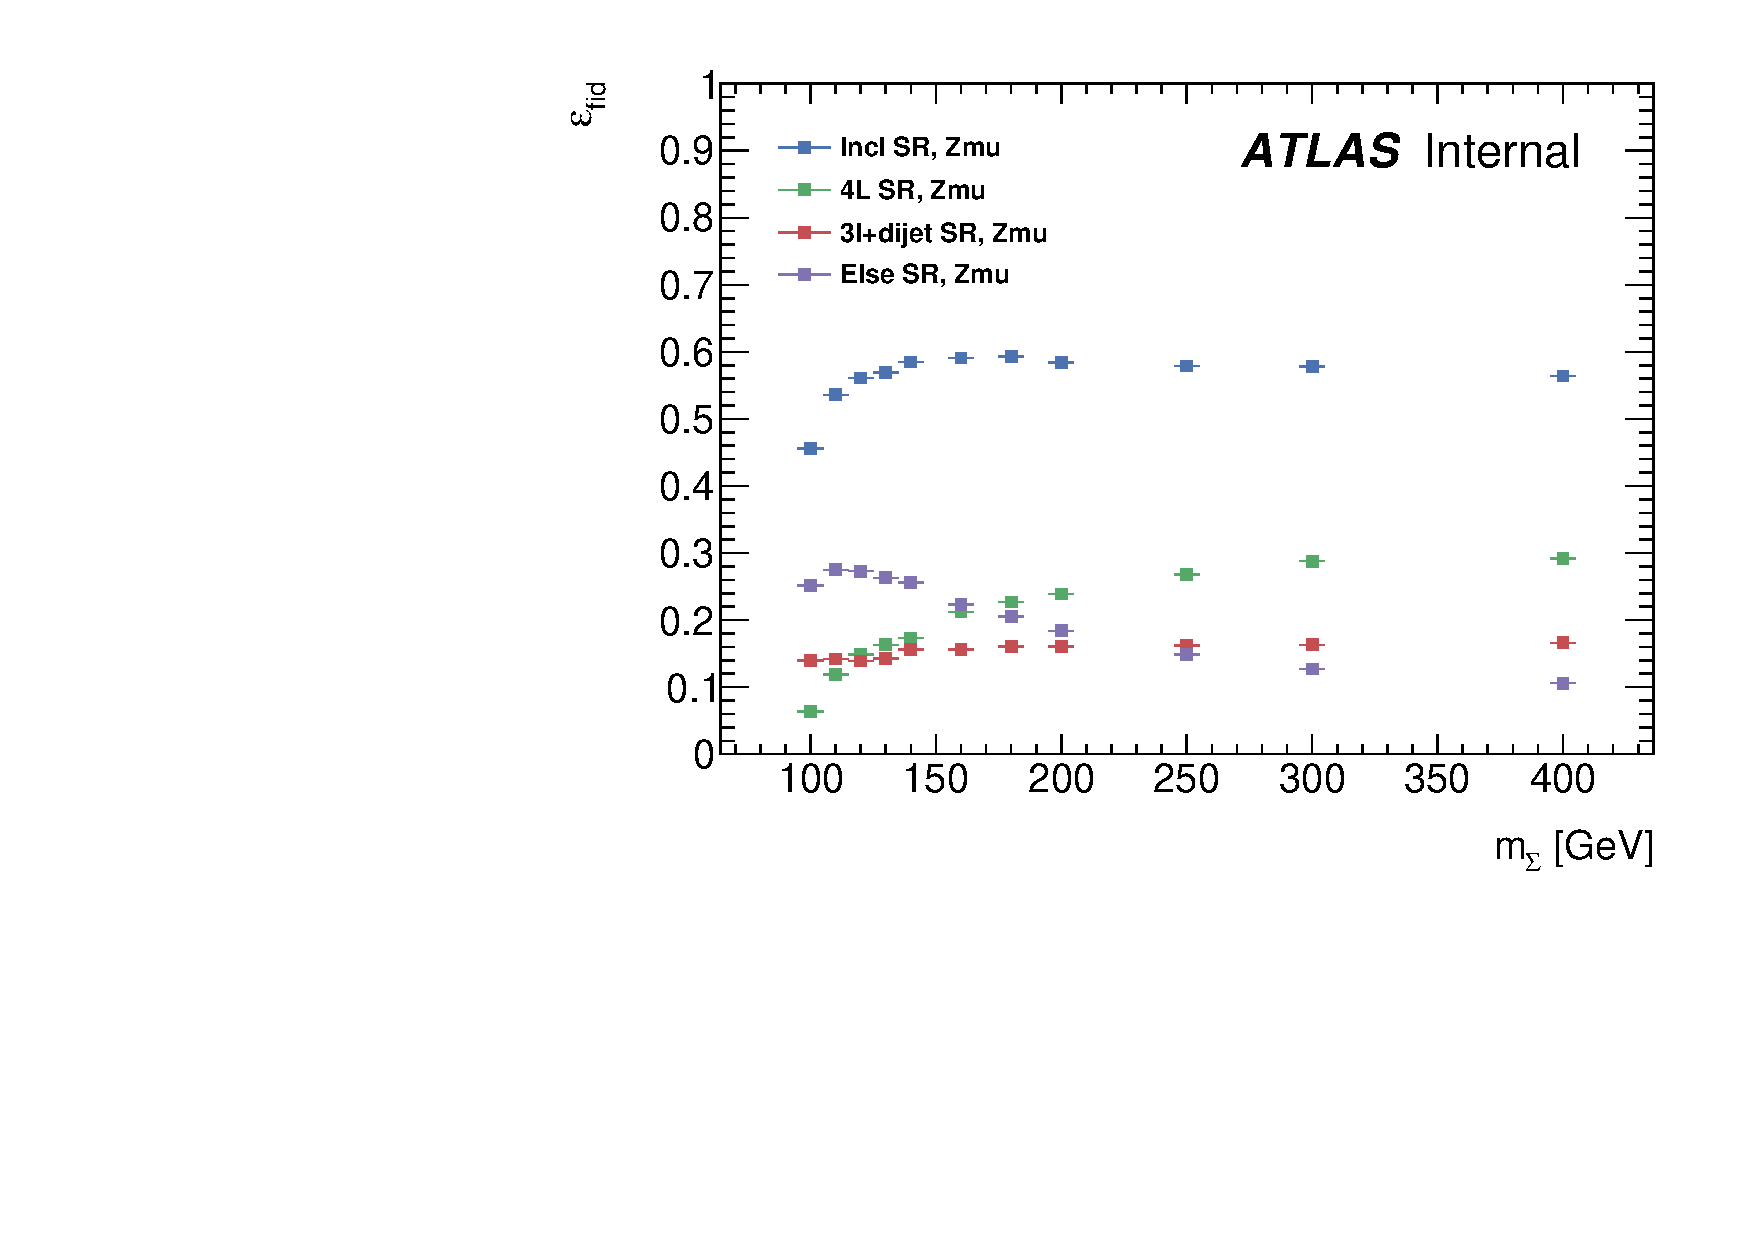
\includegraphics{figures/ch7-resonance/c_eff_fid_Zmu_VLL}}
	}
	\caption{Efficiencies of cuts defining each signal region on fiducial $Z(ll)l$ events at each simulated mass point. For the $Z+e$ signal regions, the branching fraction is set to be $BR(\Sigma\rightarrow X+e/\nu_{e})=100\%$; similarly, for the $Z+\mu$ signal regions, the branching fraction is set to be $BR(\Sigma\rightarrow X+\mu/\nu_{\mu})=100\%$.}
	\label{fig:fiducial-efficiencies-vs-mass}
\end{figure}

\section{Backgrounds}
\subsection{Background Composition}

\subsection{Systematic Uncertainties}

\subsection{Background Validation}


\section{Results and Limits}